\documentclass{article}
\usepackage[utf8]{inputenc}
\usepackage[T1]{fontenc}
\usepackage[italian]{babel}
\usepackage{geometry}
\usepackage{graphicx}
\geometry{a4paper, margin=1in}

\title{Sicurezza della Rete}
\author{}
\date{}

\begin{document}

\maketitle

La sicurezza delle reti si occupa di proteggere la comunicazione e l'integrità dei dati che transitano attraverso diverse infrastrutture. Gli argomenti principali coperti in questa sezione includono le minacce alle comunicazioni, la sicurezza wireless, gli attacchi DoS/DDoS, l'uso della crittografia, i firewall e i sistemi di rilevamento delle intrusioni (IDS/IDPS).

\section*{Concetti Base}

L'intercettazione è il primo passo di molte minacce di rete e varia drasticamente in base al mezzo trasmissivo utilizzato.

\subsection*{Mezzi Trasmissivi e Vulnerabilità Fisiche}

I cavi tradizionali sono soggetti a diverse tecniche di attacco:

\begin{itemize}
    \item \textbf{Sniffing:} Un dispositivo (packet sniffer) recupera tutti i pacchetti su una LAN. Può anche essere utilizzata una scheda di rete (NIC) riprogrammata per catturare e reinserire pacchetti nella rete.
    \item \textbf{Radiazione:} È possibile leggere i segnali irradiati dal cavo senza contatto fisico, purché l'intrusore sia vicino.
    \item \textbf{Splicing del cavo:} Consiste nel tagliare fisicamente il cavo per inserire uno sniffer.
    \item \textbf{Fibra Ottica:} Rappresenta il mezzo più sicuro poiché è immune alle radiazioni ed è quasi impossibile effettuarne lo splicing senza essere rilevati.
\end{itemize}

\subsection*{Comunicazioni Wireless e Satellitari}

Le tecnologie senza fili presentano sfide uniche. I segnali a \textbf{microonde (WiFi)} solitamente non sono schermati, facilitando l'intercettazione lungo il percorso di trasmissione, a patto di trovarsi nella linea di vista. Nelle \textbf{comunicazioni satellitari} (LEO, MEO o GEO), l'impronta di trasmissione è estremamente ampia (broadcast footprint), il che permette intercettazioni su vasta scala senza che l'attaccante venga rilevato.

\section*{Minacce alle Comunicazioni di Rete}

Le minacce possono essere classificate in tre categorie principali di danno, che influenzano la triade CIA (Riservatezza, Integrità, Disponibilità):

\begin{enumerate}
    \item \textbf{Intercettazione (Eavesdropping):} Corrisponde alla perdita di riservatezza. Le contromisure includono la crittografia (la più efficace), la sicurezza fisica delle linee, l'uso di linee dedicate e il controllo del routing.
    \item \textbf{Modifica (Integrity Failure):} Corrisponde alla perdita di integrità tramite corruzione dei dati.
    \item \textbf{Interruzione:} Corrisponde alla perdita di disponibilità o Denial of Service (DoS).
\end{enumerate}

\section*{Intercettazione: Cosa rende una rete vulnerabile a questa minaccia?}

Un utente domestico isolato o un ufficio indipendente con pochi dipendenti sono bersagli improbabili per molti attacchi. Ma se si aggiunge una rete esterna, il rischio aumenta notevolmente. Consideriamo queste caratteristiche di una rete:

\begin{itemize}
    \item anonimato
    \item molteplici punti di accesso
    \item risorse condivise
    \item sistema complesso
    \item assenza di un perimetro evidente
    \item molteplici percorsi di comunicazione
\end{itemize}

Queste caratteristiche possono portare a delle vere e proprie vulnerabilità all'intercettazione. Tra le più importanti:

\subsection*{Anonimato}

Un attaccante può sferrare un attacco da migliaia di chilometri di distanza senza mai entrare in contatto diretto con il sistema, i suoi amministratori o gli utenti. Il potenziale aggressore è così protetto da uno "scudo elettronico". L'attacco può essere fatto transitare attraverso molti altri host nel tentativo di mascherarne l'origine; inoltre, l'autenticazione tra computer non è la stessa che avviene tra esseri umani.

\subsection*{Molteplici Punti di Attacco}

Un semplice sistema informatico è un'unità autonoma in cui i controlli di accesso proteggono la riservatezza dei dati su quel singolo processore. In rete, invece, i dati o i file possono attraversare molti host prima di raggiungere l'utente. Sebbene l'amministratore di un host possa applicare politiche di sicurezza rigorose, non ha alcun controllo sugli altri nodi della rete. L'utente deve quindi fare affidamento sui meccanismi di controllo di ogni sistema attraversato; un attacco può arrivare da qualsiasi host verso qualunque altro, rendendo le grandi reti piene di punti di vulnerabilità.

\subsection*{Condivisione}

Poiché le reti abilitano la condivisione di risorse e carichi di lavoro, esse aprono l'accesso a un numero di utenti molto superiore rispetto ai computer singoli. Cosa ancora più grave, l'accesso è concesso a più sistemi contemporaneamente, rendendo i controlli di accesso pensati per sistemi isolati spesso inadeguati in un contesto di rete.

\subsection*{Complessità del Sistema}

Un sistema operativo è un software estremamente complicato e garantire una sicurezza affidabile su un sistema di grandi dimensioni è difficile, se non impossibile, specialmente se non è stato progettato nativamente per la sicurezza. Una rete coinvolge due o più sistemi operativi potenzialmente diversi tra loro, rendendo il sistema di controllo di rete inevitabilmente più complesso di quello di un singolo computer.

Oggi, un comune laptop ha una potenza di calcolo superiore a quella dei computer da ufficio di vent'anni fa. L'attaccante può sfruttare questa potenza a proprio vantaggio, facendo eseguire al computer della vittima parte dei calcoli necessari all'attacco stesso. La maggior parte degli utenti non ha idea di quali processi siano attivi in background mentre utilizza il PC, e questa complessità generale diminuisce la fiducia nella sicurezza della rete.

\subsection*{Perimetro Sconosciuto}

L'espandibilità di una rete implica intrinsecamente un'incertezza riguardo ai suoi confini. Un singolo host può fungere da nodo per due reti differenti; di conseguenza, le risorse di una rete diventano accessibili anche agli utenti dell'altra. Sebbene una vasta accessibilità sia generalmente considerata un vantaggio operativo, la presenza di questo gruppo di utenti sconosciuti, non controllati e potenzialmente malintenzionati rappresenta un grave svantaggio per la sicurezza.

Un problema analogo sorge quando è possibile aggiungere nuovi host alla rete in modo dinamico. Ogni nodo deve essere progettato per reagire alla potenziale presenza di nuovi host non affidabili. La \textbf{Figura} evidenzia le criticità nella definizione dei confini:

\vspace{0.5cm}

\noindent \begin{minipage}{0.48\textwidth}
    \begin{itemize}
        \item Un utente sulla \textbf{rete D} potrebbe non essere consapevole delle connessioni provenienti dalle \textbf{reti A e B}.
        \item Il router centrale appartiene simultaneamente alle reti \textbf{A, B, C ed E}.
        \item \textbf{Il dilemma della sicurezza:} se queste reti adottano regole di sicurezza differenti, a quali di esse deve conformarsi il dispositivo di instradamento?
    \end{itemize}
\end{minipage}
\hfill
\begin{minipage}{0.48\textwidth}
    \centering
    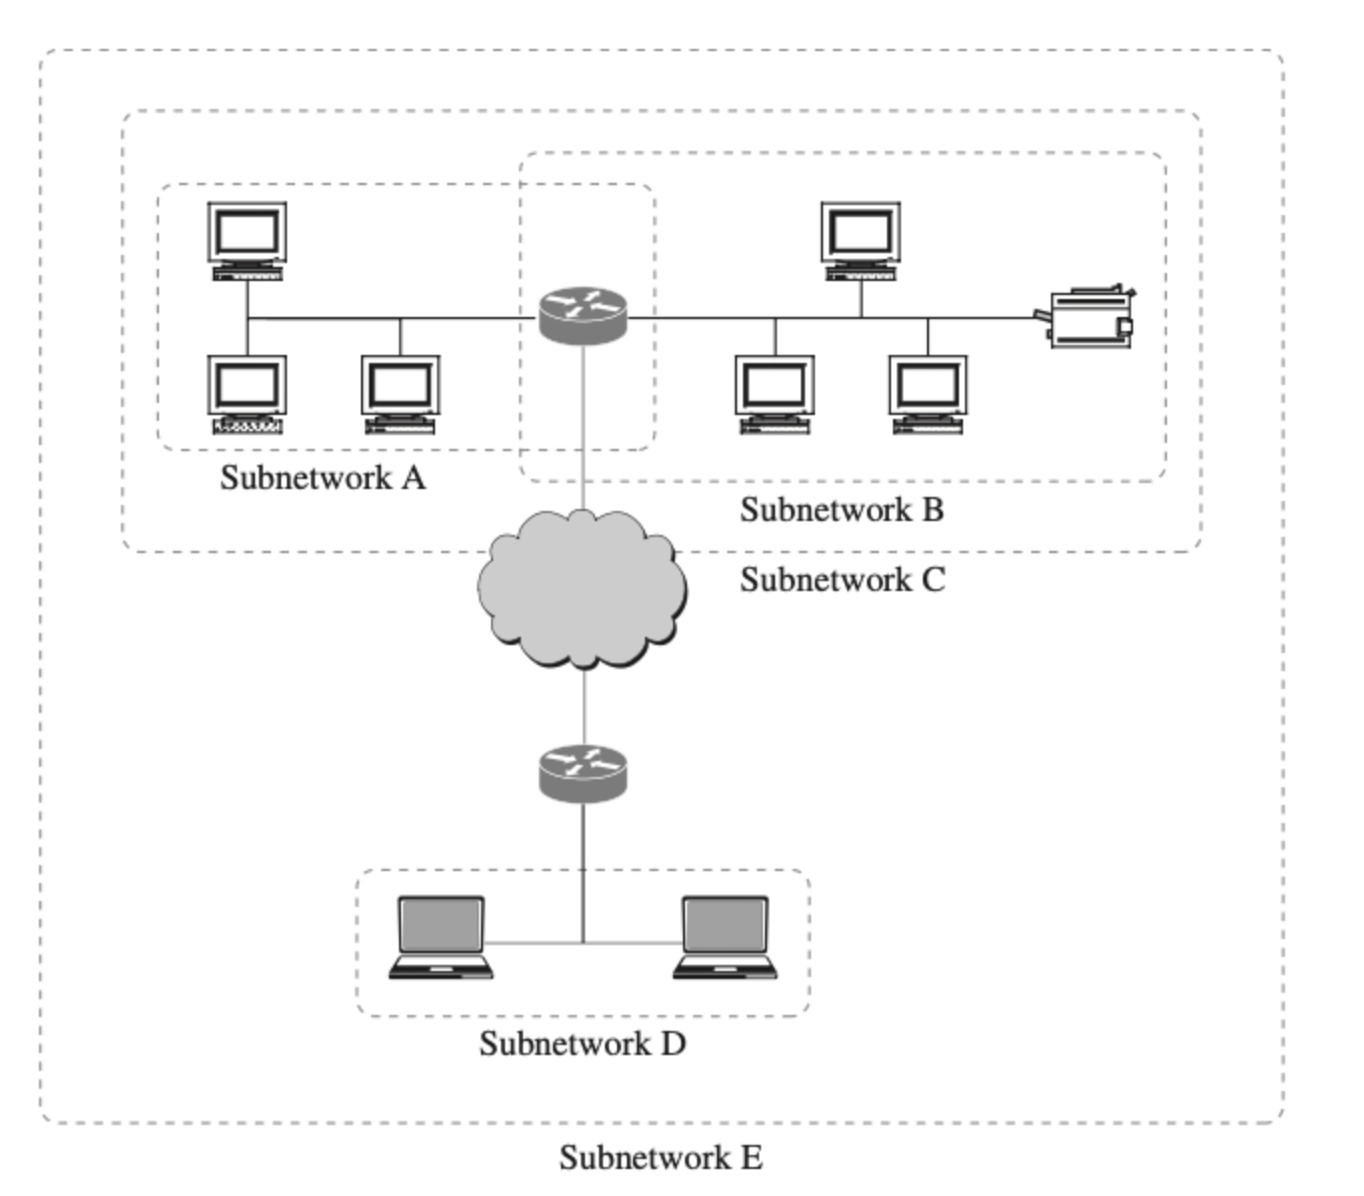
\includegraphics[width=\textwidth]{Screenshot 2026-05-05 alle 15.15.25.png}
\end{minipage}

\vspace{0.8cm}

\subsection*{Percorsi Sconosciuti}

\begin{center}
    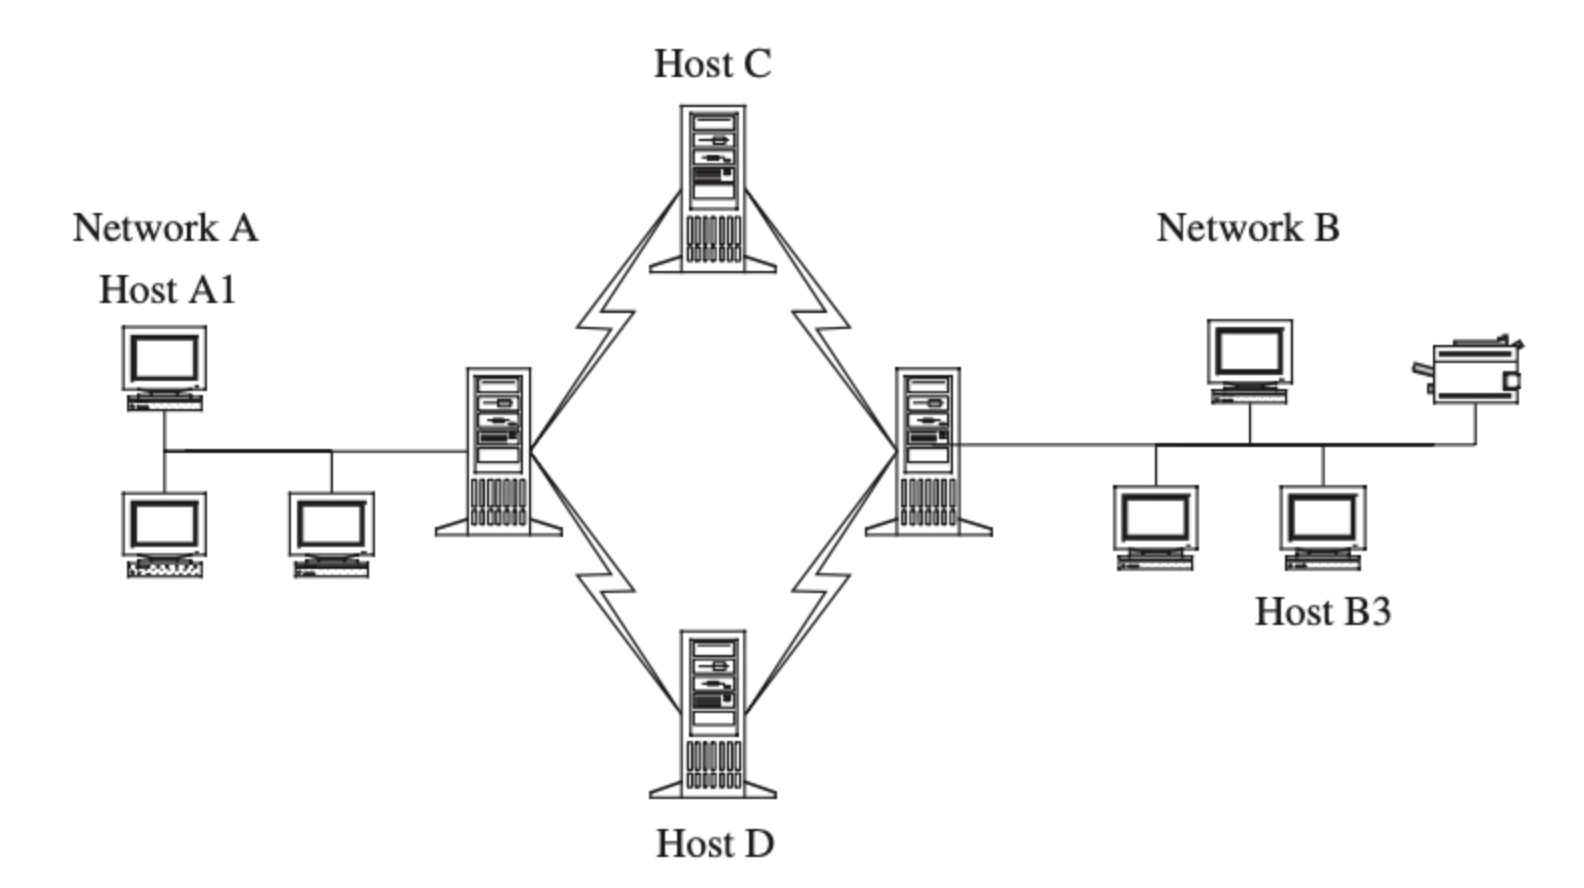
\includegraphics[width=0.7\textwidth]{Screenshot 2026-05-05 alle 15.15.33.png}
\end{center}

Come illustrato nella \textbf{Figura} esistono spesso molteplici percorsi che collegano un host a un altro all'interno di una rete complessa. Supponiamo che l'utente sull'\textbf{host A1} desideri inviare un messaggio all'utente sull'\textbf{host B3}. Tale messaggio potrebbe essere instradato attraverso l'\textbf{host C} o l'\textbf{host D} prima di giungere a destinazione. In questo scenario, l'host C potrebbe garantire un livello di sicurezza accettabile, mentre l'host D potrebbe esserne privo. Il punto cruciale è che gli utenti di rete hanno raramente il controllo sul percorso fisico o logico (routing) seguito dai propri messaggi. Questa incapacità di controllare l'instradamento è uno dei fattori determinanti nel fenomeno dell'intercettazione dei segnali, inclusi quelli della telefonia mobile.

\subsection*{Modifica: Corruzione dei Dati e Attacchi di Replay}

La corruzione dei dati avviene quando una comunicazione viene alterata durante la trasmissione. Questo può avvenire tramite \textbf{attacchi di modifica} (cambiando dati in transito), \textbf{inserimento} (creando nuovo contenuto falso) o \textbf{replay}.

\subsubsection*{Attacchi di Modifica: Errori di Sequenziamento e Sostituzione}

Un errore di sequenziamento si verifica quando un frammento successivo di uno stream arriva prima di uno precedente. Sebbene il TCP gestisca l'ordinamento, le applicazioni non sempre rilevano manipolazioni malevole in questo ambito. La \textbf{sostituzione}, invece, avviene inserendo pezzi di una comunicazione in un'altra; è particolarmente efficace con comunicazioni formattate dove l'attaccante sa esattamente quale campo modificare.

\subsubsection*{L'Attacco di Replay}

\noindent \begin{minipage}{0.48\textwidth}
    In un attacco di replay, dati legittimi vengono intercettati e riutilizzati senza modifiche. L'attaccante non ha bisogno di conoscere il contenuto o il formato del messaggio: ad esempio, un messaggio crittografato che autorizza una transazione bancaria può essere inviato due volte per ottenere un doppio addebito.
\end{minipage}
\hfill
\begin{minipage}{0.48\textwidth}
    \centering
    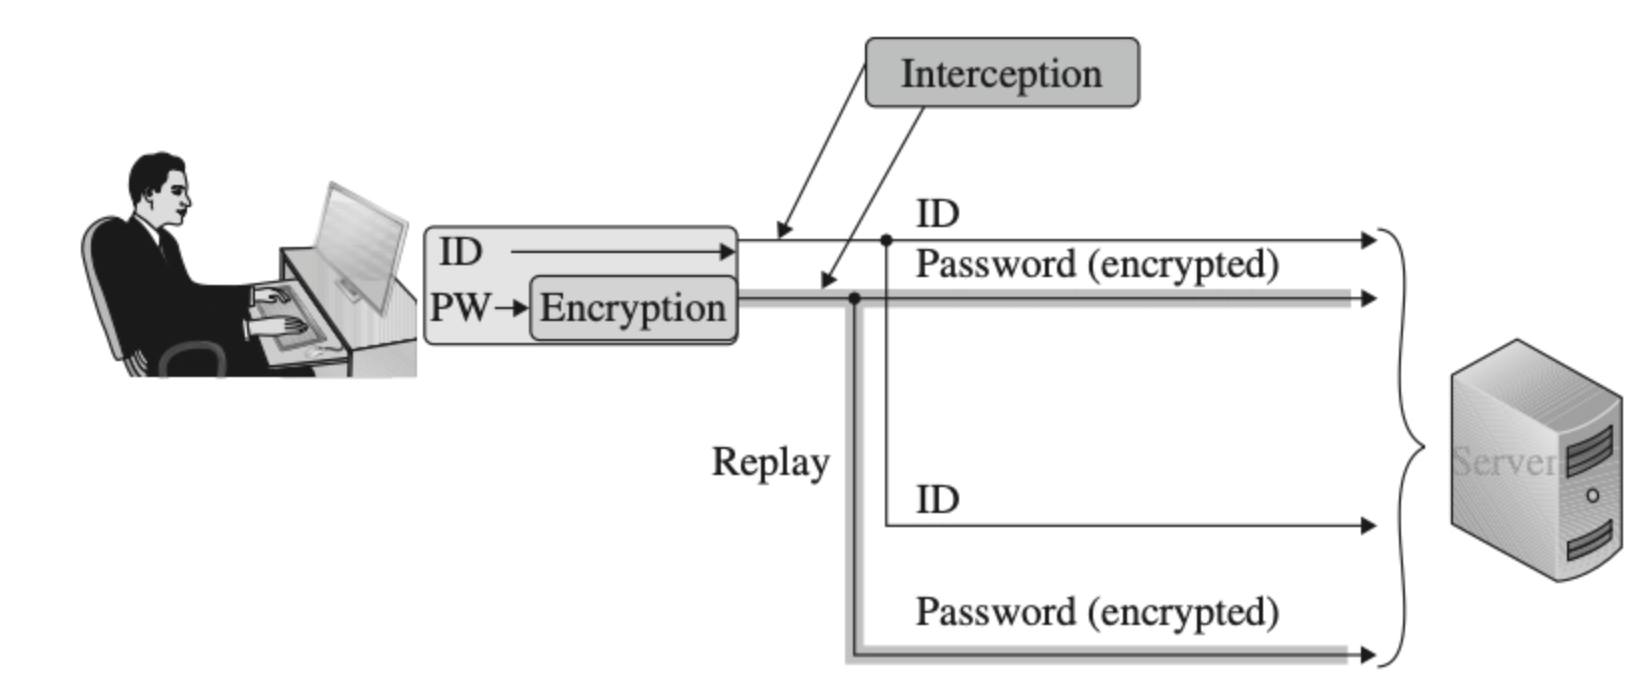
\includegraphics[width=\textwidth]{Screenshot 2026-05-05 alle 15.15.43.png}
\end{minipage}

\vspace{0.3cm}
\begin{itemize}
    \item \textbf{Difesa:} La contromisura principale è l'uso di \textbf{numeri di sequenza}. Il destinatario tiene traccia dell'ultimo numero ricevuto e accetta solo messaggi con un identificativo strettamente superiore.
\end{itemize}

\subsection*{Interruzione: Perdita di Servizio}

L'interruzione del servizio può derivare da guasti hardware (contrastati con la ridondanza) o da errori di configurazione del routing. Un esempio emblematico è il \textbf{guasto di Facebook del 2021}, causato da un comando errato di riconfigurazione BGP che ha reso l'intera rete FB invisibile su Internet, impedendo persino l'accesso fisico agli uffici perché i badge dipendevano dalla rete stessa. Altre cause includono la domanda eccessiva di risorse o i guasti indotti da malware.

\vspace{0.8cm}

\section*{Port Scanning}

Il \textbf{Port Scanning} rappresenta una delle fasi più critiche e preliminari di qualsiasi operazione di sicurezza, sia essa difensiva che offensiva. Può essere definito come l'attività di mappatura della topologia, dell'hardware e delle componenti software di un determinato segmento di rete. Nell'anatomia di un attacco informatico, la scansione delle porte agisce come una "sonda" (probe). L'obiettivo principale dell'attaccante è determinare quali servizi siano attivi e quali ulteriori attacchi potrebbero avere successo su quel particolare bersaglio.

\begin{itemize}
    \item \textbf{Port Scanner:} È un programma che, dato un indirizzo IP, riporta quali porte rispondono alle query.
    \item \textbf{CVE (Common Vulnerabilities and Exposures):} Attraverso la scansione, è possibile identificare vulnerabilità note associate a specifici servizi, spesso catalogate nel database MITRE.
    \item \textbf{Nmap:} È lo standard de facto per questa attività. Nmap non si limita a elencare le porte aperte, ma identifica il servizio supportato e, spesso, l'ID dell'utente (owner) del demone che fornisce tale servizio.
\end{itemize}

\vspace{0.5cm}

\subsection*{Analisi dei Risultati: "Hints" e Informazioni Estratte}

Un'attività di scansione, sia essa manuale o automatizzata, fornisce preziosi indizi che un attaccante può utilizzare per scalare i propri privilegi o personalizzare un exploit.

\subsubsection*{Scansione Manuale (Esempio Telnet)}

\noindent \begin{minipage}{0.48\textwidth}
    È possibile tentare una connessione manuale (ad esempio tramite \texttt{telnet} sulla porta 110 per il servizio POP) per ottenere il cosiddetto "banner" del server. Questo semplice passaggio rivela informazioni cruciali:
\end{minipage}
\hfill
\begin{minipage}{0.48\textwidth}
    \centering
    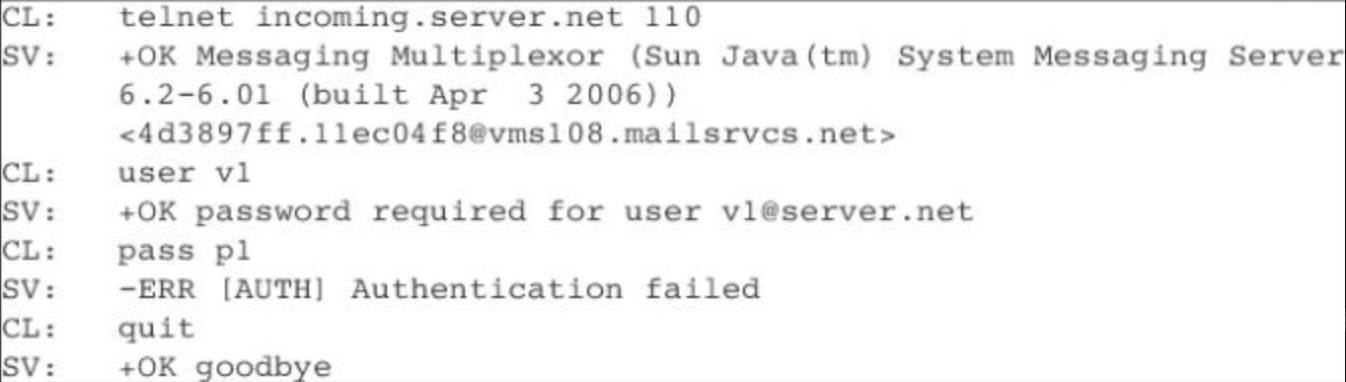
\includegraphics[width=\textwidth]{Screenshot 2026-05-05 alle 15.15.57.png}
\end{minipage}

\vspace{0.3cm}
\begin{enumerate}
    \item \textbf{Stato del servizio:} Conferma che il servizio è "UP" e funzionante.
    \item \textbf{Versione del software:} Il banner può esporre la versione esatta (es. \textit{Sun Java System Messaging Server 6.2}).
    \item \textbf{Esistenza di utenti:} Le risposte del server a tentativi di login possono confermare l'esistenza di specifici account nel sistema.
\end{enumerate}

\subsubsection*{Analisi Automatizzata con Nmap}

\noindent \begin{minipage}{0.48\textwidth}
    Una scansione Nmap completa è molto più esaustiva e permette di determinare con precisione la "superficie di attacco" del target.
    
    \vspace{0.3cm}
    \textbf{Cosa rivela Nmap:}
    \begin{itemize}
        \item Quali porte standard o servizi stanno rispondendo (es. HTTP sulla porta 80, MySQL sulla 3306).
        \item Il \textbf{Sistema Operativo} installato sul target (es. identificazione di una distribuzione CentOS).
        \item Le \textbf{applicazioni e le versioni} specifiche presenti, permettendo di mappare il software direttamente alle vulnerabilità CVE note.
    \end{itemize}
\end{minipage}
\hfill
\begin{minipage}{0.48\textwidth}
    \centering
    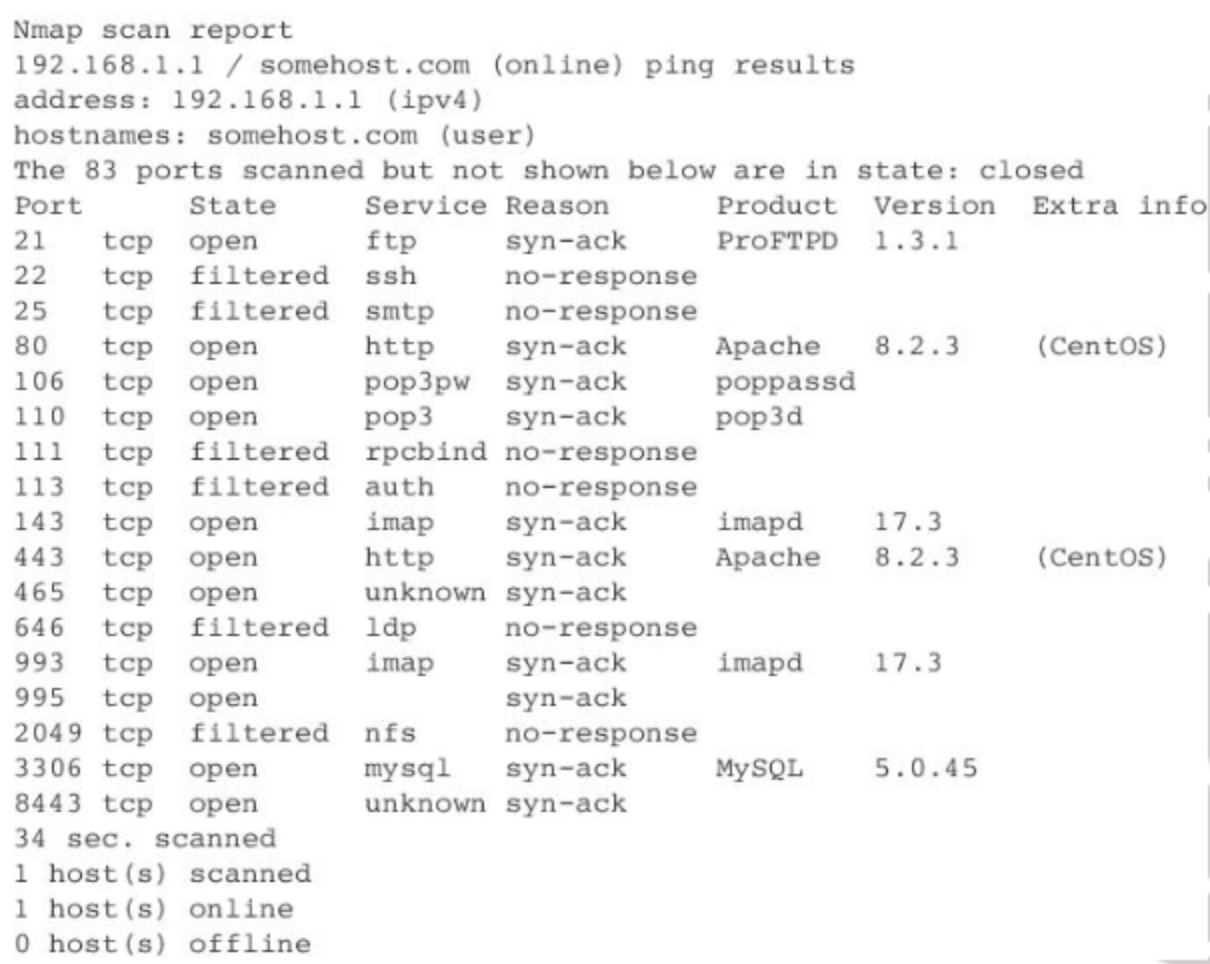
\includegraphics[width=\textwidth]{Screenshot 2026-05-05 alle 15.16.07.png}
\end{minipage}

\vspace{0.8cm}

\subsection*{Scansione di Rete e Topologia Fisica}

Il port scanning non si limita a singoli host, ma può essere esteso a interi segmenti di rete per comprenderne la struttura logica e fisica. Un indicatore fondamentale in questo senso è la \textbf{latenza}. Quando i tempi di latenza per diversi dispositivi scansionati risultano molto simili tra loro, è ragionevole dedurre che essi si trovino probabilmente sullo \textbf{stesso segmento di rete}. Questo tipo di analisi permette agli amministratori (o agli attaccanti) di mappare la vicinanza fisica dei server all'interno di un data center.

\begin{center}
    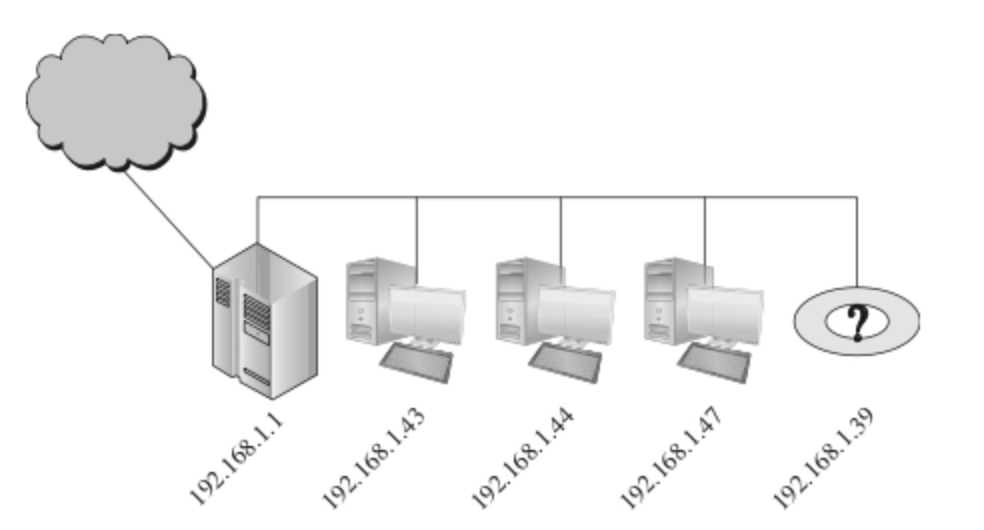
\includegraphics[width=0.7\textwidth]{Screenshot 2026-05-05 alle 15.16.16.png}
\end{center}

\section*{Sicurezza delle reti Wireless}

Nelle reti WiFi, le singole unità di dati trasmesse sono chiamate "frame". Ogni frame si scompone in tre campi principali: l'header MAC, il payload contenente i dati e la sequenza di controllo FCS (Frame Check Sequence). L'header MAC svolge un ruolo cruciale per la gestione del traffico, contenendo informazioni di dimensione fissa tra cui il tipo di frame (che può essere di controllo, di gestione o dati) e i bit che ne determinano la direzione rispetto all'access point. All'interno dell'header troviamo anche controlli per la frammentazione e l'ordine dei pacchetti, il bit WEP per segnalare la crittografia, e fino a quattro indirizzi MAC, che servono a identificare univocamente il mittente, il destinatario e gli eventuali punti di filtraggio del traffico. I frame di gestione regolano le connessioni tra i dispositivi. Ad esempio, un access point trasmette periodicamente un frame chiamato "Beacon" per annunciare la propria presenza nella rete e trasmettere parametri fondamentali come il timestamp e l'identificativo. Questo identificativo è noto come SSID (Service Set Identifier) ed è indispensabile per distinguere una rete wireless dall'altra in una stessa area. È importante notare che spesso, di default, l'SSID corrisponde a un numero di serie univoco assegnato in fabbrica. Altri frame di gestione importanti includono le richieste di autenticazione, in cui una scheda di rete si fa riconoscere, e le richieste di associazione, mediante le quali client e access point concordano le capacità di interazione, inclusi i parametri crittografici per stabilire la sessione.

\subsection*{Le Vulnerabilità del Protocollo WiFi}

La natura stessa della comunicazione radio espone il WiFi a molteplici minacce riguardo la riservatezza, l'integrità e la disponibilità del servizio. Per quanto riguarda l'integrità, il rischio risiede nel fatto che un attaccante provvisto di forti ricevitori radio WiFi può intercettare una comunicazione e prendere il sopravvento sul flusso dati, poiché questi ricevitori tendono a dare priorità al segnale più forte ricevuto. Sotto l'aspetto della disponibilità, la rete può subire disservizi a causa di guasti hardware o software, interferenze ambientali che portano alla perdita di pacchetti e ritardi per la ritrasmissione, oppure sovraccarichi quando le richieste superano la capacità di ricezione. Infine, la disponibilità è minacciata dai "rogue network connections" o hotspot pubblici, i quali, pur offrendo un servizio apparentemente funzionante, garantiscono spesso un livello di sicurezza assai limitato. Il protocollo standard del WiFi per consentire l'accesso dei dispositivi presenta criticità in ogni sua fase. Il ciclo si basa su un beacon pubblico intercettabile da chiunque, seguito da una fase di autenticazione che, in modalità base, non è per nulla rigorosa e accetta qualsiasi dispositivo. L'ultima fase, l'associazione, è altrettanto debole poiché un access point potrebbe accettare di associarsi senza restrizioni.  A gravare sulla situazione contribuisce la gestione dell'SSID: in modalità aperta (Open Mode), questo identificativo viaggia in chiaro su ogni pacchetto e raramente cambia, fornendo all'attaccante un'informazione riutilizzabile per impersonare l'access point a cui l'utente sta cercando di connettersi.  Un'ulteriore debolezza di fondo è il MAC spoofing, per cui un sistema operativo malevolo può mascherarsi dietro il MAC address fittizio di un'altra scheda di rete, ingannando gli access point che fanno uso delle liste degli indirizzi autorizzati per l'autenticazione.

\subsection*{L'Evoluzione della Sicurezza: Da WEP a WPA3}

\subsubsection*{WEP}

Il WEP è stato originariamente concepito per restituire alle comunicazioni senza fili la stessa privacy di quelle cablate. Il meccanismo prevede una chiave di crittografia condivisa tra client e access point. Per l'autenticazione, l'access point invia al client un numero casuale (RN); il client deve cifrarlo con la chiave condivisa e rispedirlo, dimostrando la propria identità. Tuttavia, si è rivelato una contromisura completamente inefficace contro le minacce di impersonificazione o intercettazione. I difetti principali del WEP sono:

\begin{itemize}
    \item \textbf{Chiave di crittografia debole e statica:} Il WEP utilizza chiavi da 64 o 128 bit, ma i primi 24 bit sono occupati dal vettore di inizializzazione (IV), riducendo la reale forza della chiave a soli 40 o 104 bit. Inoltre, la chiave è statica: gli utenti tendono a usare la stessa chiave per molto tempo, permettendo agli attaccanti di raccogliere abbastanza traffico per poterla dedurre.
    \item \textbf{Processo crittografico vulnerabile:} Il WEP non utilizza l'algoritmo RC4 in modo diretto, ma genera una sequenza di chiavi combinata con i dati tramite una funzione XOR. Se un attaccante indovina una porzione del testo in chiaro, può risalire alla chiave; inoltre, i difetti noti dell'algoritmo RC4 consentono di violare il WEP in pochi minuti.
    \item \textbf{Collisioni del vettore di inizializzazione (IV) e controlli difettosi}: I 24 bit dell'IV compiono un ciclo prevedibile di circa 16 milioni di combinazioni, rendendo facile per un attaccante testarle tutte rapidamente. Inoltre, il controllo di integrità dei messaggi usa un algoritmo noto: un hacker può modificare il contenuto del messaggio, ricalcolare il valore di controllo e ingannare il destinatario.
    \item \textbf{Mancanza di autenticazione:}  Il WEP non richiede alcuna autenticazione. Qualsiasi dispositivo in grado di fornire il giusto SSID e un indirizzo MAC valido (facilmente falsificabile) viene considerato legittimo. In sintesi, il design del WEP è inaccettabile poiché non usa la crittografia in modo efficace e non protegge dalle modifiche intenzionali.
\end{itemize}

\subsubsection*{WPA}

Per riparare ai danni del WEP, è stato introdotto il WPA. La sua principale innovazione consiste nell'uso del Temporal Key Integrity Program (TKIP), un sistema che rende la chiave non statica e la cambia automaticamente per ogni pacchetto scambiato. L'autenticazione viene delegata al protocollo EAP (Extensible Authentication Protocol), e al vecchio RC4 si affianca la più robusta crittografia AES, oltre a introdurre controlli di integrità a 64 bit crittografati. Una sessione WPA si instaura tramite un "four-way handshake" utile a generare in maniera sicura le chiavi di crittografia e integrità in entrambi i lati della connessione. Tuttavia, anche il WPA ha le sue crepe:

\begin{itemize}
    \item \textbf{Man-in-the-Middle e Autenticazione incompleta:}Sfruttando la falsificazione dell'indirizzo MAC (spoofing), un attaccante può intromettersi tra il client e l'access point inviando falsi messaggi di disassociazione, prendendo poi il posto dell'utente legittimo. Questo accade perché il client non ha modo di essere assolutamente certo che l'access point a cui si sta autenticando sia quello reale.
    \item \textbf{Ricerca esaustiva (Attacchi a dizionario):}  Per facilità d'uso, molte reti WPA permettono l'inserimento di password (passphrase). Poiché gli esseri umani tendono a scegliere password deboli, gli hacker possono usare attacchi a dizionario per indovinarle, sebbene il processo di conversione della chiave del WPA sia volutamente lento per ostacolare questi tentativi.
    \item \textbf{Attacco Chopchop:} I ricercatori hanno dimostrato che il meccanismo TKIP (progettato per essere compatibile con i vecchi hardware WEP) può essere eluso "tagliando" e sostituendo singoli byte di un blocco cifrato per dedurne la chiave. Tuttavia, questo attacco non è efficace contro il WPA2 che utilizza l'algoritmo AES.
\end{itemize}

Nel complesso, le vulnerabilità del WPA si verificano in casi ristretti; scegliendo chiavi di crittografia lunghe e casuali, il protocollo rimane adeguatamente sicuro. Nel 2018, la Wi-Fi Alliance ha introdotto il WPA3. Questa nuova versione mantiene la struttura di base, ma elimina del tutto il rischio degli attacchi a dizionario contro le password, impiega chiavi crittografiche ancora più lunghe e supporta tecniche di associazione semplificate che non richiedono l'inserimento di password indovinabili. L'autore conclude ricordando che, più che i difetti dei protocolli Wi-Fi, il problema reale è la quantità di dati sensibili che gli utenti trasmettono senza protezioni a livello applicativo.

\section*{Denial of Service (DoS)}

Un attacco Denial of Service (DoS) rappresenta un tentativo di sconfiggere la "disponibilità", il terzo pilastro fondamentale della sicurezza informatica. A differenza della riservatezza e dell'integrità, che tendono a essere concetti binari (i dati sono privati/integri oppure non lo sono), la disponibilità possiede molte più sfumature. Un servizio negato può variare da una completa perdita di accesso fino a un inaccettabile rallentamento delle risposte, configurandosi a volte come un grave danno e altre come un semplice fastidio. Le cause principali che portano alla negazione di un servizio si dividono in tre grandi categorie:

Le cause principali che portano alla negazione di un servizio si dividono in tre grandi categorie:

\begin{itemize}
    \item \textbf{Capacità insufficiente (Overload / Flooding):} Si verifica quando la domanda (il traffico) è superiore a ciò che il sistema può gestire, saturando ad esempio un collegamento di rete; questi attacchi sono noti come attacchi "volumetrici".
    \item \textbf{Accesso bloccato:} L'attaccante impedisce il funzionamento di un servizio sfruttando una vulnerabilità software per far crashare l'applicazione (application-based attack), interferendo con i meccanismi di routing della rete, disabilitando i controlli di accesso, o persino crittografando i file vitali del sistema (es. attacchi Ransomware).
    \item \textbf{Componenti non responsivi (Guasti):} L'inaccessibilità causata da fallimenti fisici dell'hardware o da errori del software, i quali possono avvenire in modo accidentale o essere indotti artificialmente.
\end{itemize}

\subsection*{Attacchi di Flooding}

La forma più primitiva di attacco DoS consiste nell'inondare (flooding) una connessione, impedendo di fatto al sistema di ricevere qualsiasi altro dato legittimo. Questo problema è spesso esacerbato dalla robustezza stessa dei protocolli TCP: in caso di congestione, se alcuni pacchetti subiscono ritardi, il protocollo trattiene quelli successivi e richiede la ritrasmissione di quelli mancanti, finendo per alimentare ulteriormente l'ingorgo.

Oltre all'abuso del TCP e dell'UDP, molti attacchi sfruttano impropriamente la suite di protocolli ICMP (Internet Control Message Protocol), normalmente utilizzata per la diagnostica di sistema e priva di applicazioni utente associate. I messaggi diagnostici maggiormente manipolati includono:

\begin{itemize}
    \item \textbf{Ping ed Echo:} Richiedono rispettivamente a una destinazione di rispondere per dimostrare la propria raggiungibilità e di rimandare indietro i dati ricevuti per testare l'affidabilità del collegamento.
    \item \textbf{Destination Unreachable e Source Quench:} Indicano rispettivamente che un indirizzo non può essere raggiunto o che la destinazione è satura, avvisando la sorgente di sospendere l'invio dei pacchetti. Poiché questi messaggi di controllo sono gestiti direttamente dallo stack di rete e operano spesso senza autenticazione, un attaccante può utilizzarli liberamente per saturare le prestazioni della rete.
\end{itemize}

Il flooding rappresenta la macro-categoria di attacco DoS ma appartenenti ad essa esistono quattro tipici attacchi:

\subsubsection*{Ping of Death}

È un attacco semplice che abusa del comando \texttt{ping}, normalmente utilizzato per testare i tempi di risposta di un host. L'attaccante invia una valanga ininterrotta di pacchetti ping (ICMP Echo Request) alla vittima. L'efficacia dipende dal "collo di bottiglia" della banda passante sulla rotta. L'attacco ha successo se la larghezza di banda dell'attaccante è superiore a quella della vittima.

\textbf{Esempio:} Se un attaccante dispone di una connessione a 100 MB e la vittima a 10 MB, i pacchetti inonderanno rapidamente la rete della vittima, saturandone completamente la banda.

% --- IMMAGINE PING OF DEATH ---
\begin{figure}[htbp]
    \centering
    % Sostituisci il nome del file all'interno delle parentesi graffe
    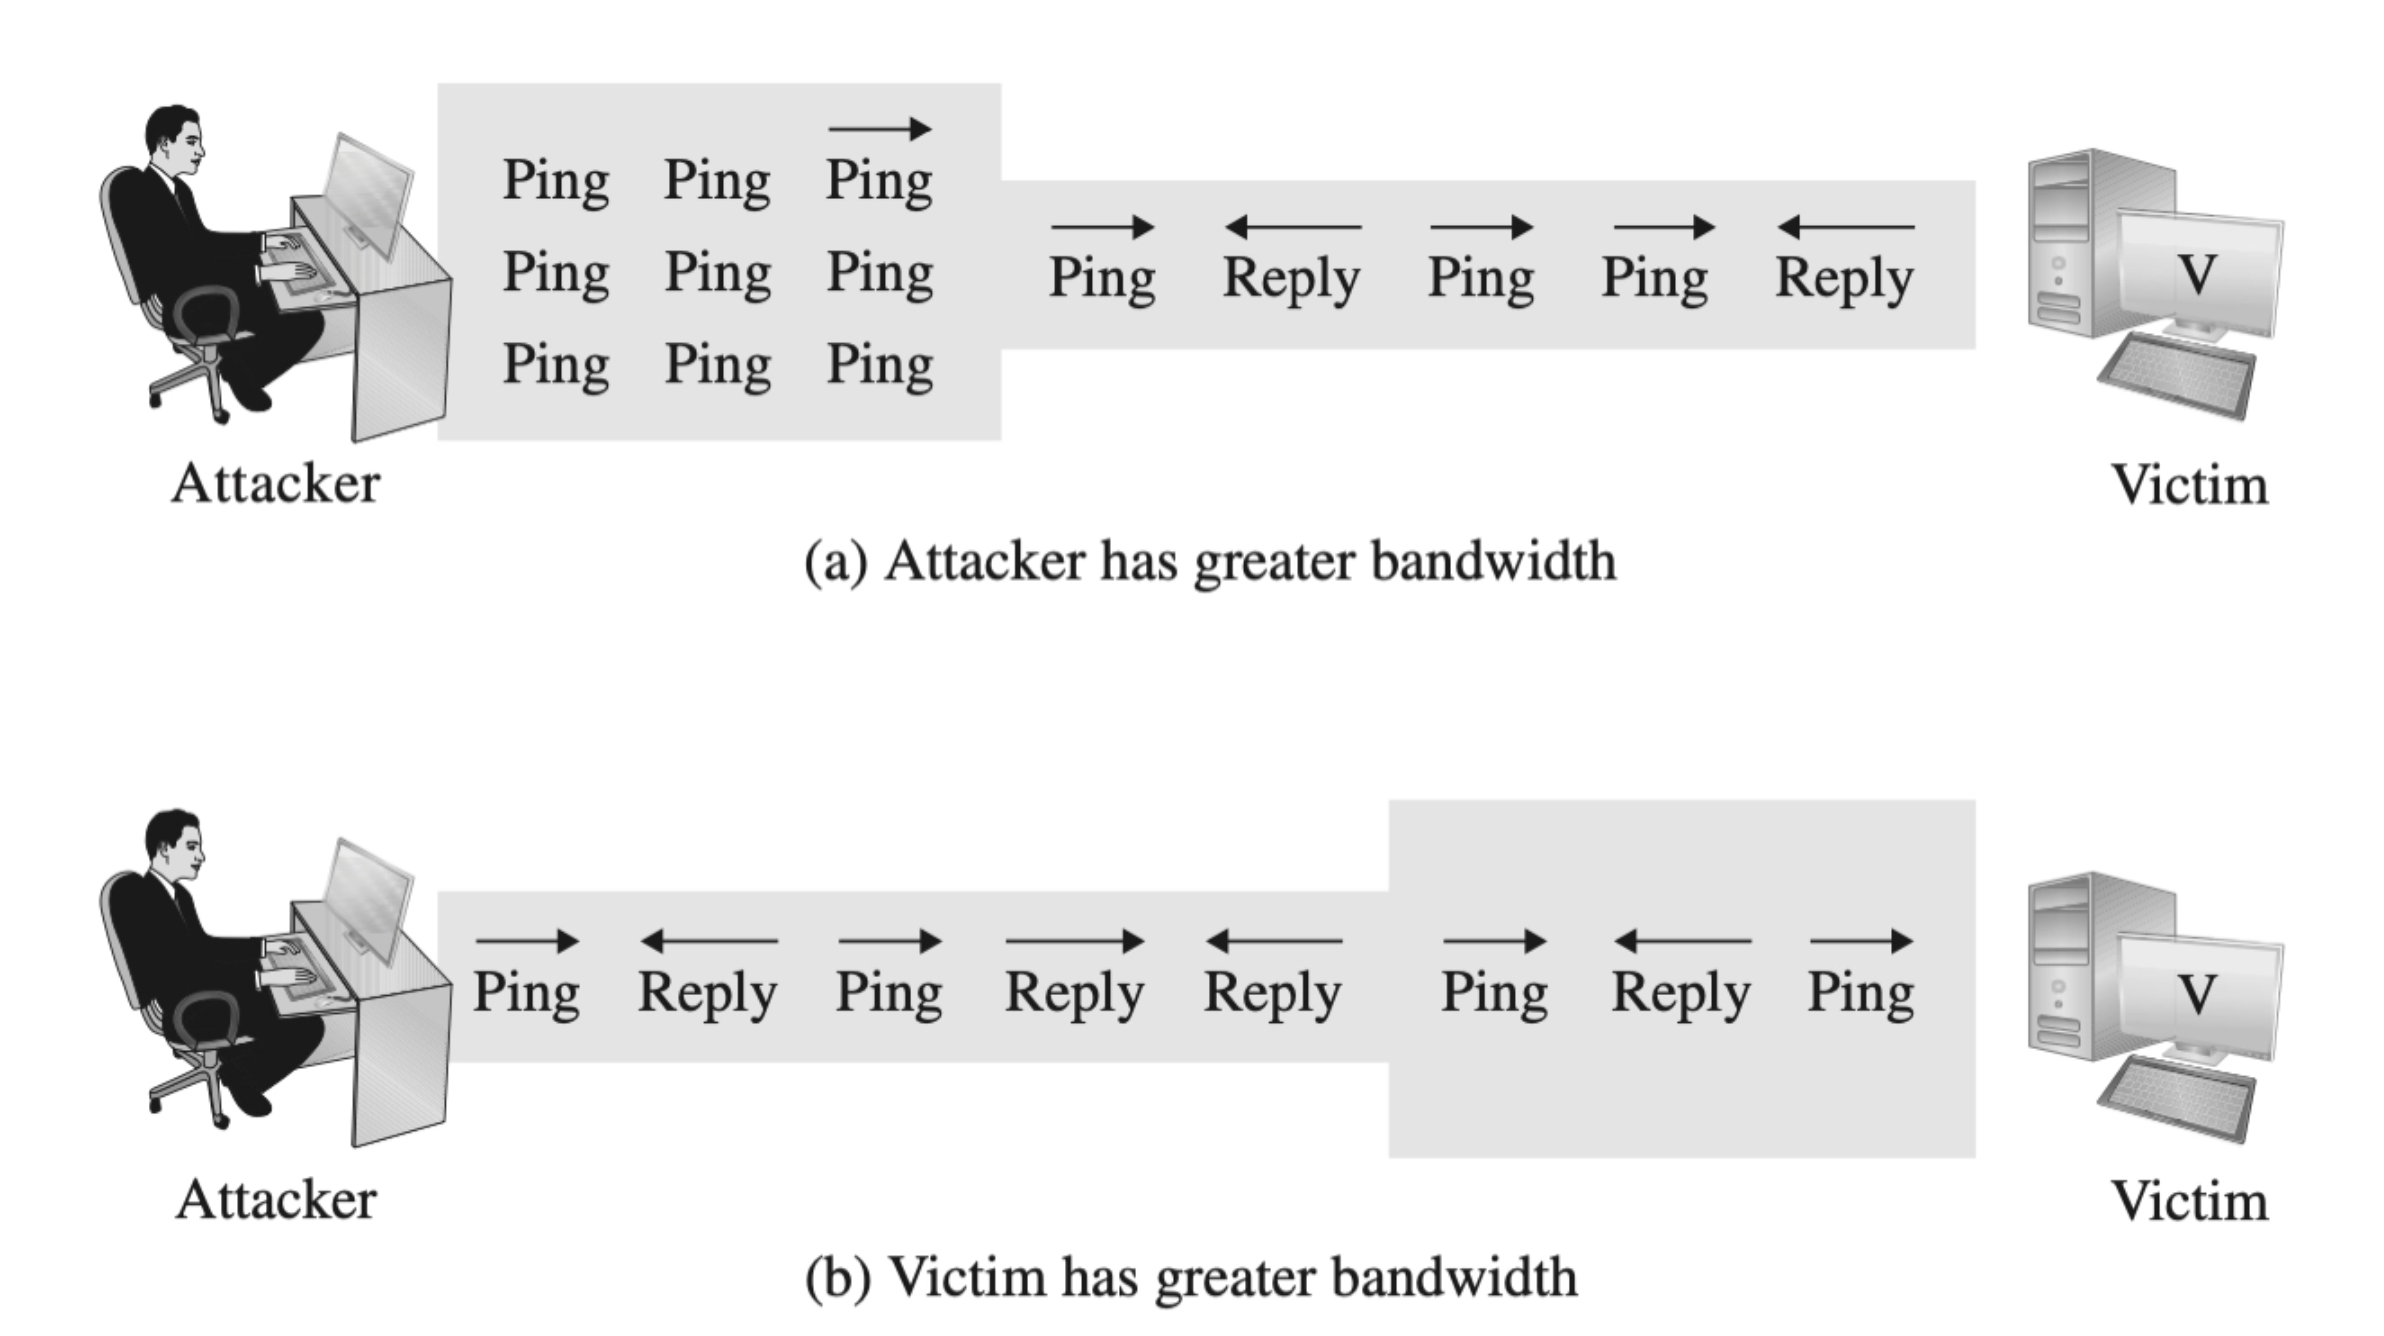
\includegraphics[width=0.8\textwidth]{Screenshot 2026-05-23 alle 11.02.53.png}
    \caption{Schema dell'attacco Ping of Death in base alla larghezza di banda.}
    \label{fig:ping_of_death}
\end{figure}

\subsubsection*{Attacco Smurf (Smurf Attack)}

Si tratta di un'evoluzione molto più devastante dell'attacco ping, basata su un principio di \textbf{amplificazione} tramite reti terze ignare. Sfrutta due "trucchi":

\begin{itemize}
    \item \textbf{Fase 1: Spoofing (Falsificazione):} L'attaccante falsifica l'indirizzo IP sorgente del pacchetto ping, inserendo l'indirizzo IP della vittima. In questo modo, chiunque riceva il pacchetto penserà che sia stata la vittima a inviarlo.
    \item \textbf{Fase 2: Broadcast:} Invece di mandare il pacchetto a un singolo host, l'attaccante lo invia all'indirizzo di \textit{broadcast} di una rete subalterna (impostando l'ultimo byte dell'indirizzo su tutti \texttt{1}). Un pacchetto broadcast viene distribuito a \textit{tutti} gli host presenti in quella sottorete.
\end{itemize}

Ogni singolo host della rete complice riceve il ping e risponde all'indirizzo sorgente (che è stato falsificato con quello della vittima). La vittima viene così inondata da una moltiplicazione massiccia di risposte simultanee.

% --- IMMAGINE SMURF ATTACK ---
\begin{figure}[htbp]
    \centering
    % Sostituisci il nome del file all'interno delle parentesi graffe
    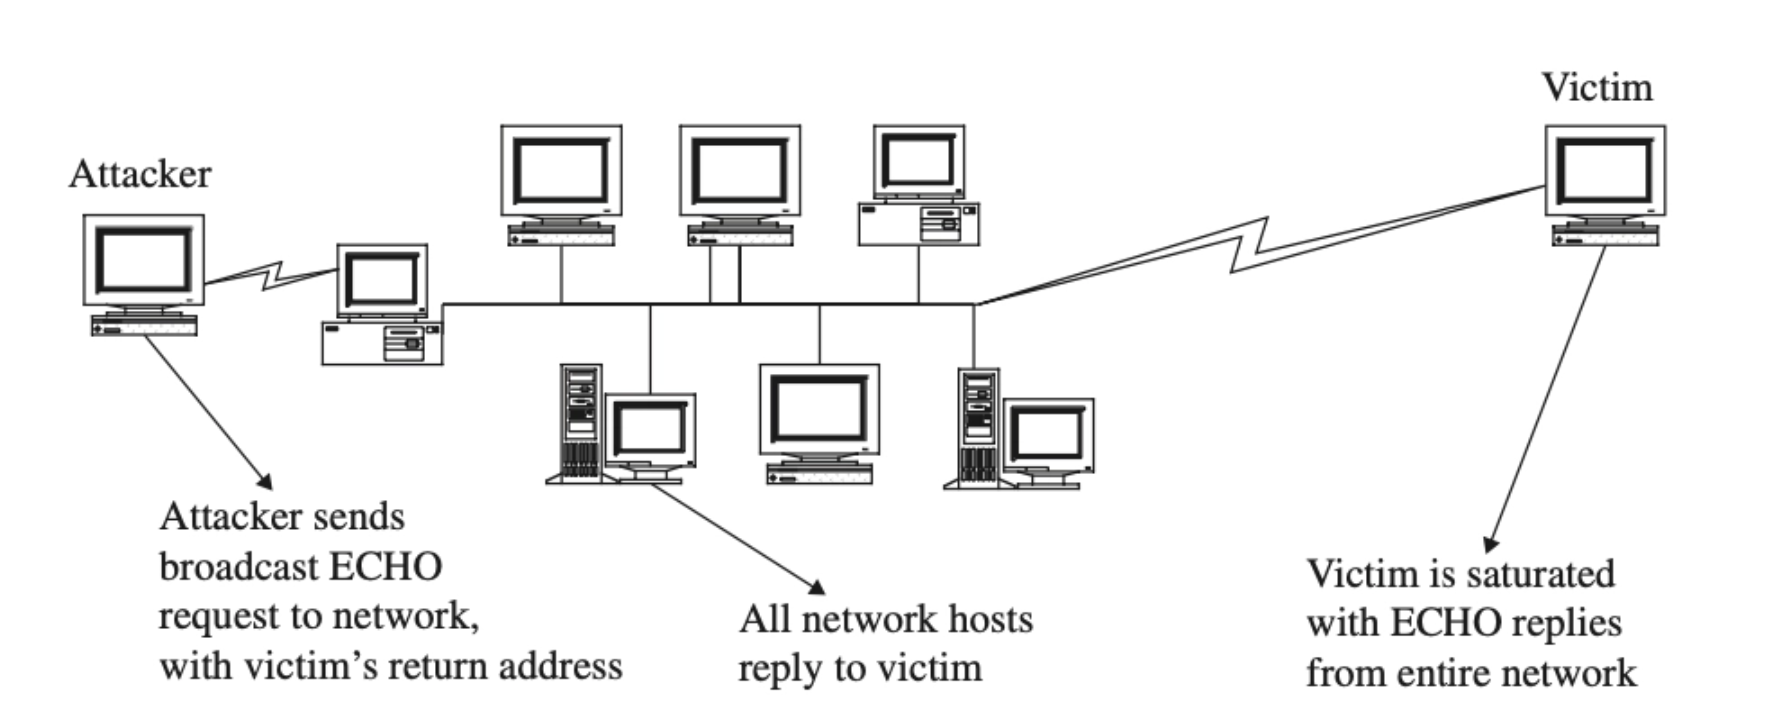
\includegraphics[width=0.8\textwidth]{Screenshot 2026-05-23 alle 11.02.58.png}
    \caption{Dinamica dell'Attacco Smurf con rete amplificatrice.}
    \label{fig:smurf_attack}
\end{figure}

\subsubsection*{Attacco Echo-Chargen}

Questo attacco crea un \textit{loop} (ciclo) infinito sfruttando due servizi di test del protocollo ICMP: \textbf{Chargen} (che genera un flusso continuo di pacchetti) ed \textbf{Echo} (che rispedisce al mittente esattamente ciò che riceve). L'attaccante prende di mira due host (A e B). Invia al servizio Chargen dell'Host A dei pacchetti richiedendo un Echo, ma \textit{falsifica} l'indirizzo sorgente facendo figurare l'Host B.

\begin{enumerate}
    \item L'Host A (tramite Chargen) genera un pacchetto e lo invia a B.
    \item L'Host B (tramite Echo) lo riceve e lo rispedisce diligentemente ad A.
    \item L'Host A lo riceve e lo rispedisce a B... come in una partita di tennis infinita.
\end{enumerate}

Le infrastrutture di rete di entrambi gli host si saturano in un ciclo senza fine. Esiste anche una variante in cui l'attaccante imposta sia la sorgente che la destinazione sull'Host B, bloccando la macchina in un loop infinito con se stessa.

% --- IMMAGINE ECHO-CHARGEN ---
\begin{figure}[htbp]
    \centering
    % Sostituisci il nome del file all'interno delle parentesi graffe
    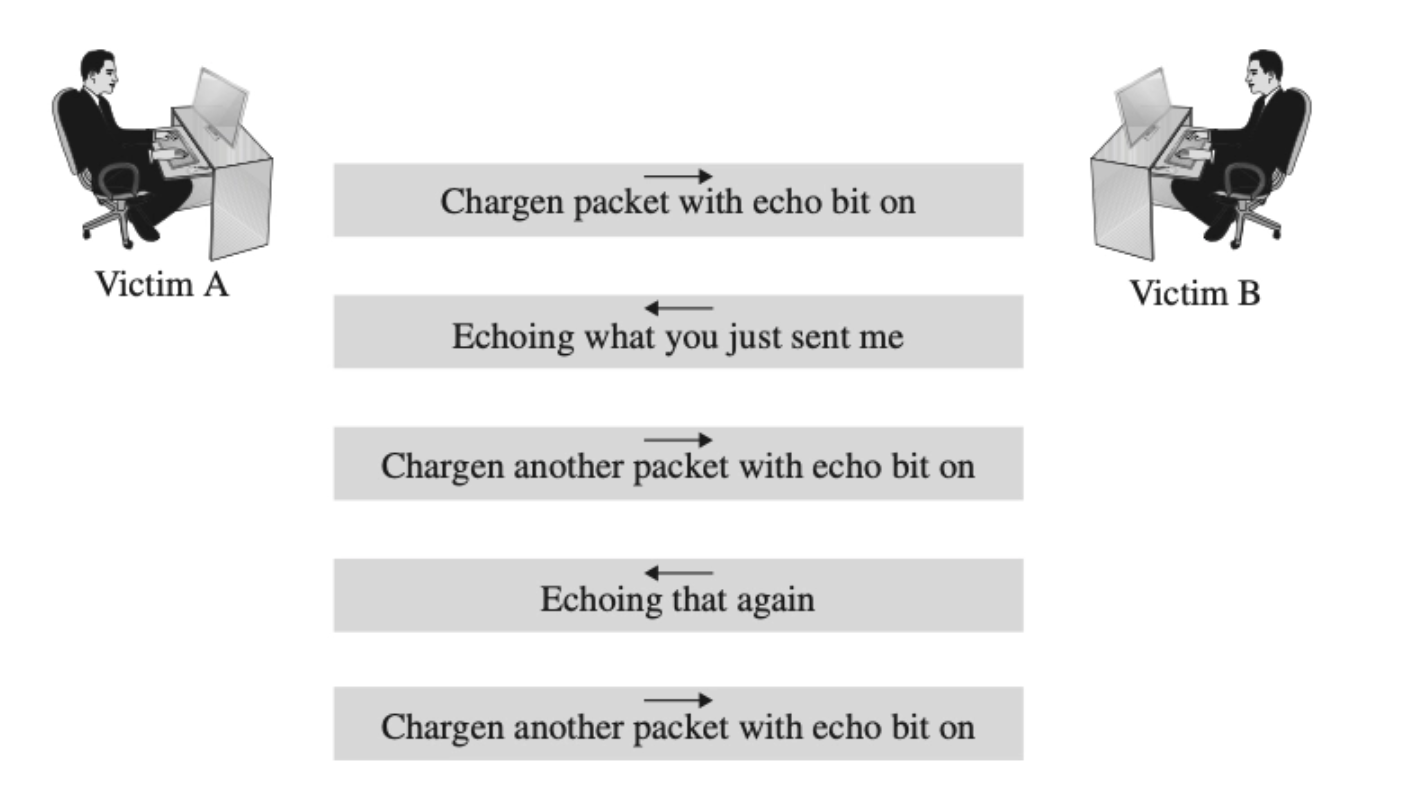
\includegraphics[width=0.8\textwidth]{Screenshot 2026-05-23 alle 11.03.06.png}
    \caption{Rappresentazione del loop nell'attacco Echo-Chargen.}
    \label{fig:echo_chargen}
\end{figure}

\subsubsection*{SYN Flood}

Il SYN Flood è un attacco molto popolare che rivolge contro la vittima la natura stessa del protocollo TCP e il suo meccanismo per stabilire le connessioni (il \textit{Three-Way Handshake}).

\textbf{Il normale Handshake TCP:}
\begin{enumerate}
    \item Il mittente invia un pacchetto \texttt{SYN} (Synchronize).
    \item Il ricevente risponde con un pacchetto \texttt{SYN-ACK}.
    \item Il mittente conferma con un pacchetto \texttt{ACK} (Acknowledge), aprendo il canale.
\end{enumerate}

Se un server riceve un \texttt{SYN} e invia un \texttt{SYN-ACK}, la connessione rimane "in sospeso" in attesa dell'\texttt{ACK} finale. Queste connessioni parziali vengono memorizzate in una coda chiamata \texttt{SYN\_RECV}. Questa coda è tipicamente molto piccola e il server aspetterà per diversi minuti prima di scartare una connessione incompleta.

\textbf{Esecuzione dell'Attacco:}
\begin{itemize}
    \item L'attaccante invia moltissime richieste \texttt{SYN} valide.
    \item Il server vittima risponde con \texttt{SYN-ACK} e alloca spazio nella coda \texttt{SYN\_RECV}.
    \item L'attaccante \textbf{non} invia mai il pacchetto \texttt{ACK} finale.
    \item La coda della vittima si riempie immediatamente. Di conseguenza, il server non può più accettare nuove connessioni da utenti legittimi (negazione del servizio).
\end{itemize}

Gli attaccanti raramente usano il loro vero indirizzo IP in un SYN Flood; utilizzano invece indirizzi di ritorno inesistenti per due motivi fondamentali:
\begin{enumerate}
    \item \textbf{Nascondere l'identità:} Per non farsi rintracciare ispezionando la coda \texttt{SYN\_RECV}.
    \item \textbf{Eludere i controlli:} Per rendere il traffico malevolo indistinguibile da quello legittimo. Quando il server invia il \texttt{SYN-ACK} a un IP inesistente, riceve un errore "ICMP Destination Unreachable". Tuttavia, poiché ICMP e TCP sono protocolli separati, questo errore di rete non comunica al gestore TCP di chiudere la connessione in sospeso.
\end{enumerate}

% --- IMMAGINE SYN FLOOD ---
\begin{figure}[htbp]
    \centering
    % Sostituisci il nome del file all'interno delle parentesi graffe
    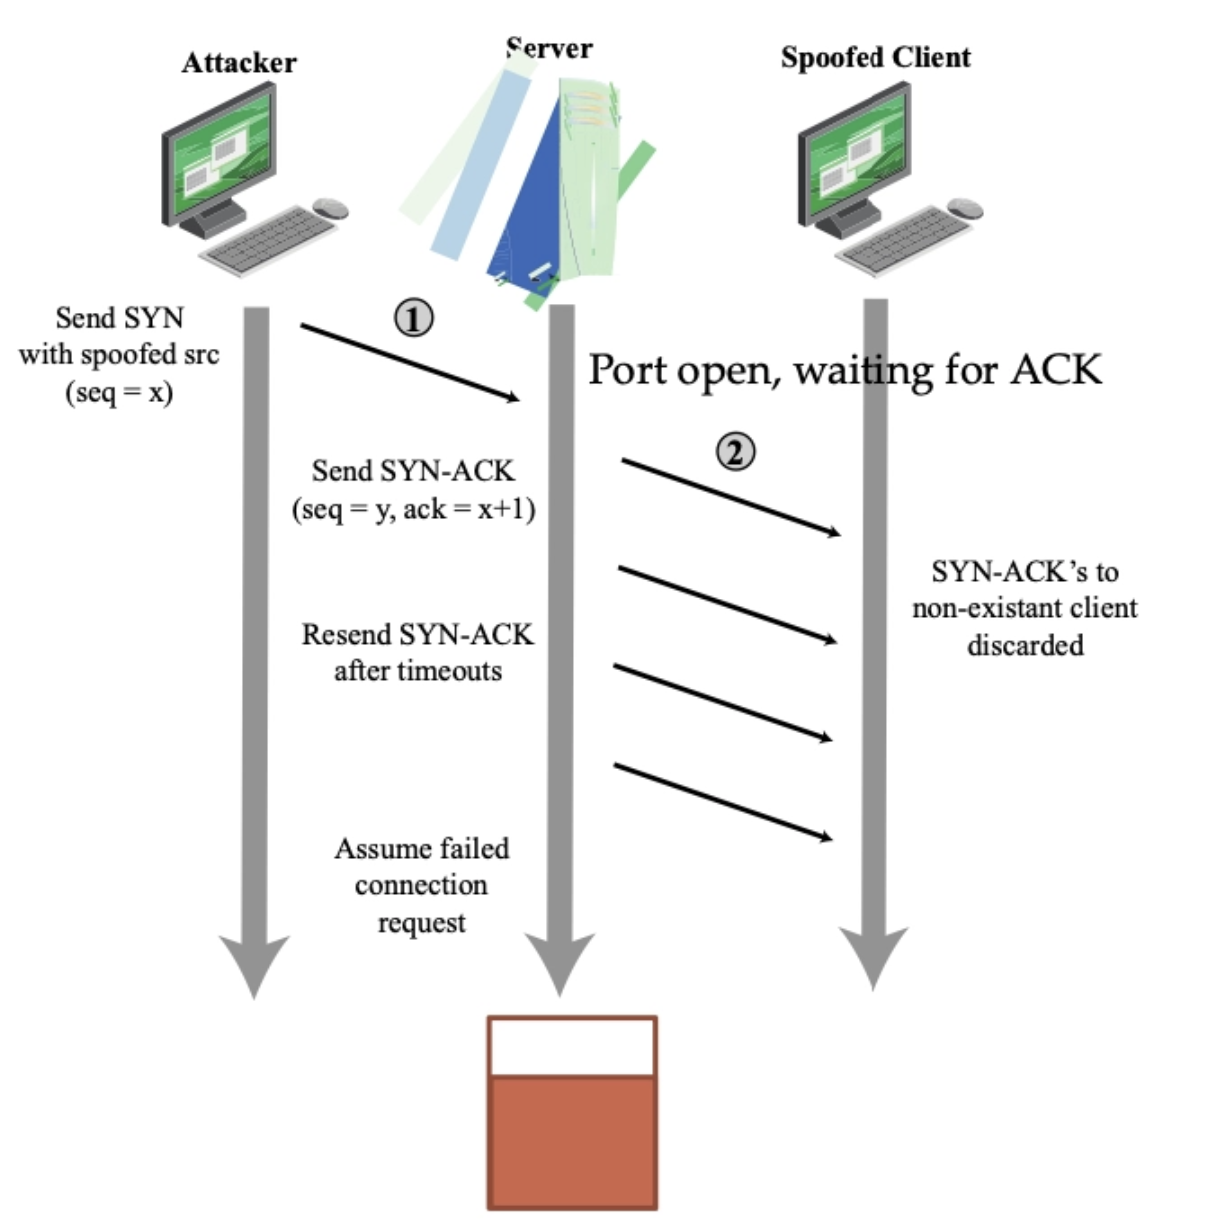
\includegraphics[width=0.7\textwidth]{Screenshot 2026-05-23 alle 11.03.15.png}
    \caption{Diagramma del flusso dell'attacco SYN Flood con IP contraffatto.}
    \label{fig:syn_flood}
\end{figure}

\subsection*{Attacchi ai "Componenti non responsivi"}

\subsubsection*{Teardrop Attack}

% --- TESTO E IMMAGINE TEARDROP AFFIANCATI ---
\vspace{0.3cm}
\noindent \begin{minipage}{0.48\textwidth}
A differenza del Ping of Death o del SYN Flood, il Teardrop non cerca di saturare la banda (Flooding). Sfrutta un difetto nel modo in cui i sistemi operativi riassemblano i pacchetti frammentati. L'attaccante invia frammenti IP con informazioni di lunghezza sovrapposte; il sistema operativo della vittima va in confusione nel tentativo di ricostruire il dato, si blocca o va in crash, causando la negazione del servizio.
\end{minipage}
\hfill
\begin{minipage}{0.48\textwidth}
    \centering
    % Sostituisci il nome del file all'interno delle parentesi graffe
    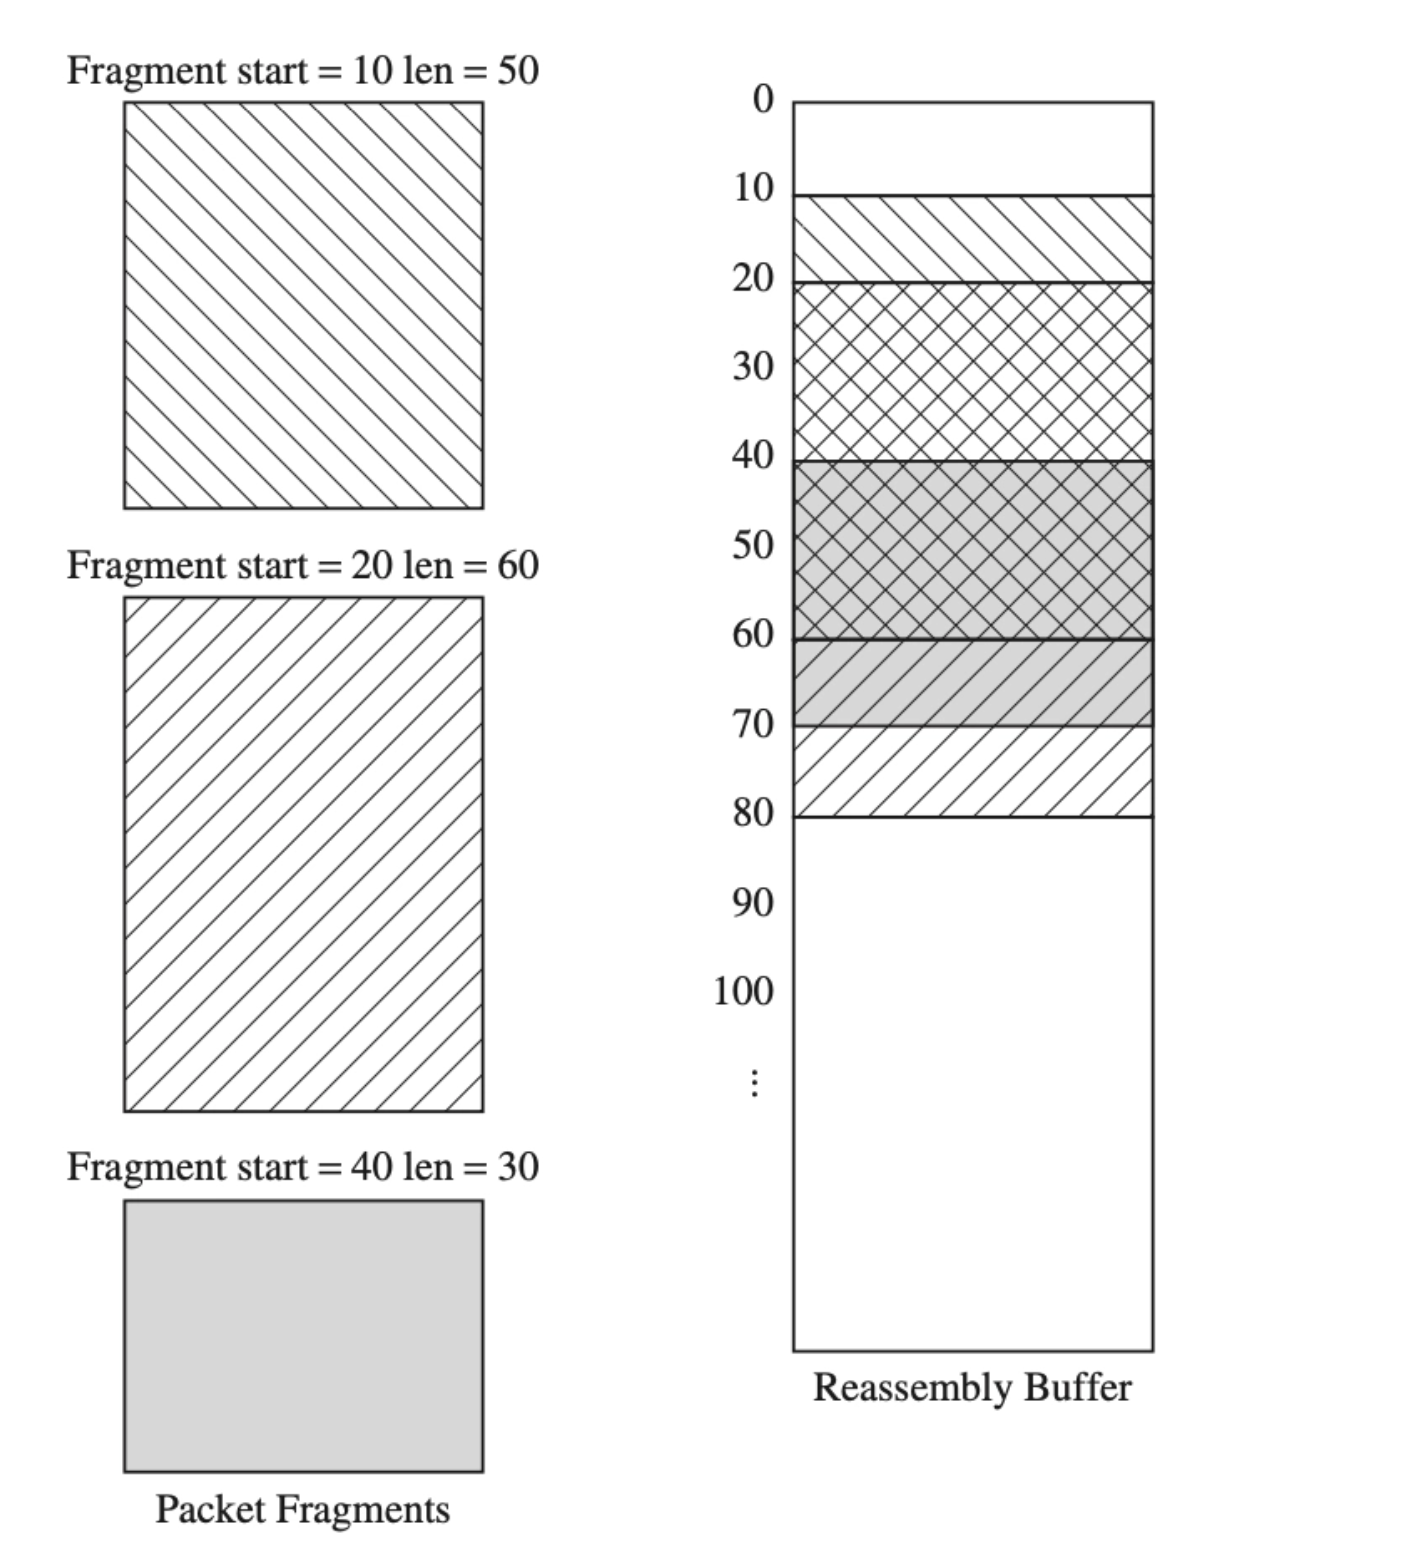
\includegraphics[width=0.9\textwidth]{Screenshot 2026-05-23 alle 11.03.22.png}
    \label{fig:teardrop}
\end{minipage}
\vspace{0.5cm}

\subsection*{Attacchi all'infrastruttura (L'accesso bloccato per vie traverse)}

Per impedire a un utente di raggiungere un servizio, non è obbligatorio abbattere il server di destinazione. Basta distruggere le "indicazioni stradali" per raggiungerlo. Questo gruppo di slide si allontana dai protocolli di trasporto (TCP/UDP/ICMP) e colpisce i protocolli di livello superiore (DNS) o di rete (Routing).

\subsubsection*{DNS Poisoning}
Se un attaccante riesce a inquinare la cache di un server DNS (Poisoning) o a mettersi in mezzo alla comunicazione (Spoofing - Man in the Middle), può reindirizzare le tue richieste legittime verso un IP inesistente o malevolo. Il server originale è perfettamente funzionante, ma il servizio ti è comunque negato.

\subsubsection*{Top-Level Domain Attacks}
Invece di colpire un singolo sito, si mira ai server che gestiscono i domini di primo livello (es. i server radice dei domini \texttt{.it} o \texttt{.com}).

\subsubsection*{Routing attacks}
Simile al concetto del DNS, ma agisce a livello di router. Alterando le tabelle di routing (usate dai router per decidere dove inviare i pacchetti), l'attaccante crea dei colli di bottiglia artificiali (instradando tutto il traffico verso un router che poi collassa) oppure crea dei "buchi neri" in cui i pacchetti vengono scartati.

\subsection*{Dirottamento e Desincronizzazione}

\subsubsection*{Session Hijack}
Qui l'obiettivo è negare o manipolare una singola connessione già stabilita. Inserendo pacchetti con numeri di sequenza falsificati, l'attaccante fa sì che il ricevente legittimo scarti i pacchetti veri (perché i numeri di sequenza non tornano più). Se i due nodi non riescono a risincronizzarsi, la sessione TCP cade, causando un DoS mirato su quella specifica comunicazione.

% --- IMMAGINE TCP HIJACK ---
\begin{figure}[htbp]
    \centering
    % Sostituisci il nome del file all'interno delle parentesi graffe
    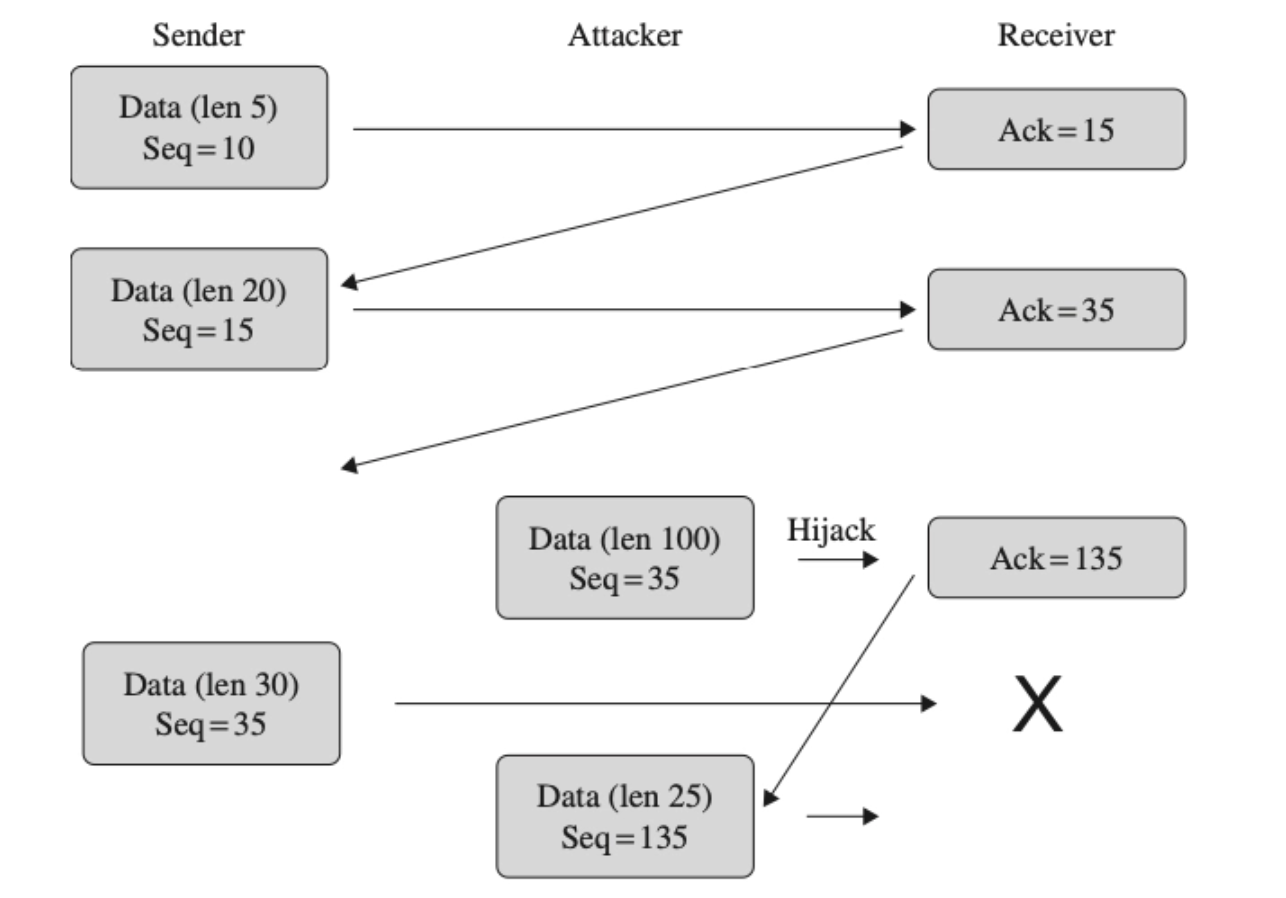
\includegraphics[width=0.8\textwidth]{Screenshot 2026-05-23 alle 11.03.31.png}
    \caption{Dinamica dell'attacco TCP Hijack tramite falsificazione dei numeri di sequenza.}
    \label{fig:tcp_hijack}
\end{figure}

\subsection*{L'Evoluzione: il DDoS}

Il Distributed Denial-of-Service (DDoS) rappresenta l'evoluzione su larga scala dei tradizionali attacchi DoS, pensata per superare un limite fisico invalicabile. In un attacco DoS standard, come il Ping of Death, l'efficacia dell'offensiva si basa su un rapporto di forza uno-a-uno: l'attaccante vince solo se possiede una larghezza di banda superiore a quella del bersaglio. Il DDoS stravolge questa dinamica trasformando lo scontro in un "molti contro uno", aggregando la potenza di calcolo e di rete di migliaia di macchine per annientare bersagli altrimenti inattaccabili.

La prima fase dell'attacco consiste nel reclutamento silente delle truppe. Tramite script automatizzati che scansionano ininterrottamente Internet alla ricerca di macchine vulnerabili, l'attaccante installa un codice malevolo (spesso un Trojan horse) sui computer di utenti ignari. Una volta infettata, la macchina diventa uno "zombie" o "bot". La caratteristica peculiare è che non danneggia in nessun modo il computer ospite. La macchina deve rimanere perfettamente in salute, connessa e operativa, affinché l'utente legittimo continui a usarla senza sospettare nulla. L'insieme di queste migliaia (o milioni) di macchine compromesse forma un'enorme rete interconnessa chiamata Botnet, pronta ad agire all'unisono.

Un esercito di tali dimensioni non può essere gestito direttamente. Per evitare di essere rintracciato e per garantire la sopravvivenza della rete, l'attaccante progetta una struttura gerarchica e ridondante. L'ideatore dell'attacco comunica solo con un livello intermedio di nodi "Master", i quali a loro volta gestiscono i server di Comando e Controllo (C\&C). Sono questi server C\&C a impartire direttamente gli ordini alla massa di bot. Questa intera struttura è progettata per essere altamente resiliente. I bot comunicano tra loro e con i Master attraverso canali ordinari (come IRC o reti peer-to-peer); se una parte della rete viene isolata o un server C\&C viene abbattuto dai difensori, i percorsi di comunicazione ridondanti permettono alla Botnet di riorganizzarsi senza interruzioni.

Quando giunge il momento prestabilito, i server C\&C inviano il segnale di via libera. Improvvisamente, le migliaia di zombie lanciano l'offensiva simultaneamente contro l'unica vittima designata. La vera criticità di questo attacco, oltre alla mole immensa di traffico generato, è la flessibilità tattica: non tutti i bot devono usare la stessa arma. L'attaccante può configurare la Botnet in modo che un gruppo saturi la rete della vittima con attacchi \textit{Smurf}, mentre un'altra divisione esaurisce le risorse dei server tramite \textit{SYN Flood} o \textit{Echo-Chargen}. Il bersaglio si ritrova così a dover fronteggiare contemporaneamente vulnerabilità diverse provenienti da innumerevoli direzioni, rendendo le normali strategie di difesa inefficaci.

\section*{Le Contromisure}

Nel resto di questo capitolo prenderemo in considerazione tre categorie di controlli: innanzitutto, come è facile immaginare, il noto controllo della crittografia è uno strumento efficace per preservare sia la riservatezza che l'integrità nelle reti. Descriveremo a livello architetturale come la crittografia può essere utilizzata e introdurremo due applicazioni specifiche della crittografia alle reti. Introdurremo poi uno strumento di protezione della rete chiamato firewall, che in realtà non è altro che un'istanza del noto monitor di riferimento. Concluderemo il capitolo con un altro dispositivo, chiamato sistema di rilevamento o protezione dalle intrusioni, che monitora il traffico di rete per identificare e contrastare specifiche minacce informatiche.

\subsection*{Crittografia di Rete}

La crittografia può essere impiegata in una rete attraverso due modalità generali: di collegamento (\textit{link encryption}) ed \textit{end-to-end}. Queste due modalità svolgono funzioni diverse e presentano punti di forza e debolezze differenti. Possono persino essere utilizzate insieme, anche se farlo porta a una certa ridondanza.

\subsubsection*{Link Encryption}

La crittografia di collegamento (link encryption) è una tecnica di sicurezza che opera ai livelli inferiori del modello OSI (livello 1 o 2), cifrando i dati un attimo prima che vengano immessi nel mezzo di comunicazione fisico e decifrandoli non appena raggiungono il nodo di rete successivo. Il meccanismo fondamentale prevede che i dati viaggino in chiaro (plaintext) attraverso i livelli superiori del sistema, per poi essere protetti esclusivamente lungo la singola tratta fisica. Questa architettura introduce però una vulnerabilità specifica: affinché la comunicazione proceda, ogni router o switch intermedio deve obbligatoriamente rimuovere la cifratura per leggere le informazioni di instradamento, esponendo temporaneamente il contenuto del messaggio all'interno del nodo stesso. Di conseguenza, questa soluzione risulta ideale e molto efficace quando la linea di trasmissione esterna, come i cavi condivisi che collegano due città, rappresenta il punto di maggiore vulnerabilità, ma presuppone necessariamente che tutti gli host intermedi attraversati siano intrinsecamente sicuri e affidabili. Il grande vantaggio di questa tecnologia, nonostante l'esposizione nei nodi intermedi, risiede nella sua completa trasparenza: essendo elaborata in modo estremamente rapido da dispositivi hardware dedicati, la cifratura di collegamento risulta totalmente invisibile all'utente finale, alle applicazioni e al sistema operativo, agendo silenziosamente come un servizio di rete di base alla stregua del routing o del controllo degli errori di trasmissione.

% --- IMMAGINE LINK ENCRYPTION ---
\begin{figure}[htbp]
    \centering
    % Sostituisci il nome del file all'interno delle parentesi graffe
    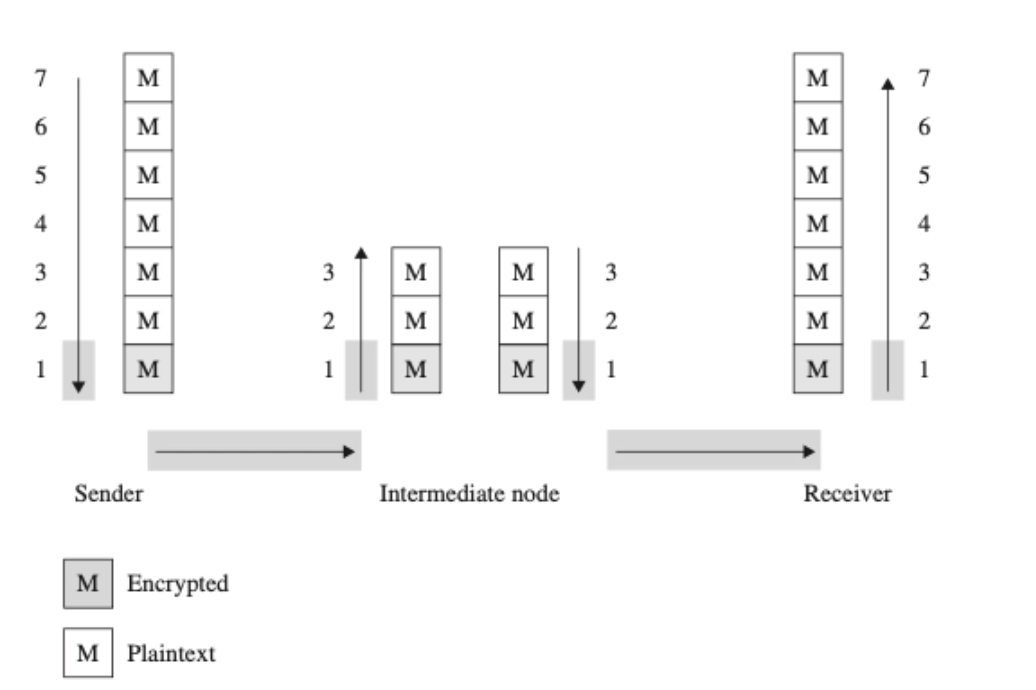
\includegraphics[width=0.7\textwidth]{Screenshot 2026-05-23 alle 11.03.40.png}
    \caption{Schema del modello OSI applicato alla Link Encryption.}
    \label{fig:link_encryption}
\end{figure}

\subsubsection*{End-to-End Encryption}

La crittografia end-to-end fornisce sicurezza da un'estremità all'altra di una trasmissione. Può essere applicata tra un utente e un host tramite un dispositivo hardware, oppure, più comunemente, viene eseguita ai livelli più alti, solitamente da un'applicazione al livello 7 del modello OSI (sebbene a volte avvenga ai livelli 5 o 6). Poiché la crittografia precede tutte le elaborazioni di instradamento (routing) e trasmissione dei livelli sottostanti, il messaggio viene trasmesso in forma cifrata attraverso l'intera rete. È importante notare che solo la porzione dei dati (il payload) del messaggio viene protetta, mentre le intestazioni (header) rimangono in chiaro; tuttavia, spesso gli header non contengono informazioni sensibili quanto i dati stessi. Questa modalità risolve le potenziali vulnerabilità presenti nei livelli inferiori del modello di trasferimento. Se un livello inferiore dovesse fallire nel preservare la sicurezza ed esporre i dati ricevuti, la riservatezza (confidentiality) di questi ultimi non verrebbe messa in pericolo. Quando si utilizza questa crittografia, i messaggi inviati attraverso vari host intermedi rimangono costantemente protetti contro la divulgazione (disclosure) durante tutto il transito. Di conseguenza, anche se un messaggio si trova costretto ad attraversare nodi potenzialmente insicuri lungo il percorso tra il mittente (nodo A) e il destinatario (nodo B), il suo contenuto informativo resta illeggibile e sicuro.

% --- IMMAGINE END-TO-END ENCRYPTION ---
\begin{figure}[htbp]
    \centering
    % Sostituisci il nome del file all'interno delle parentesi graffe
    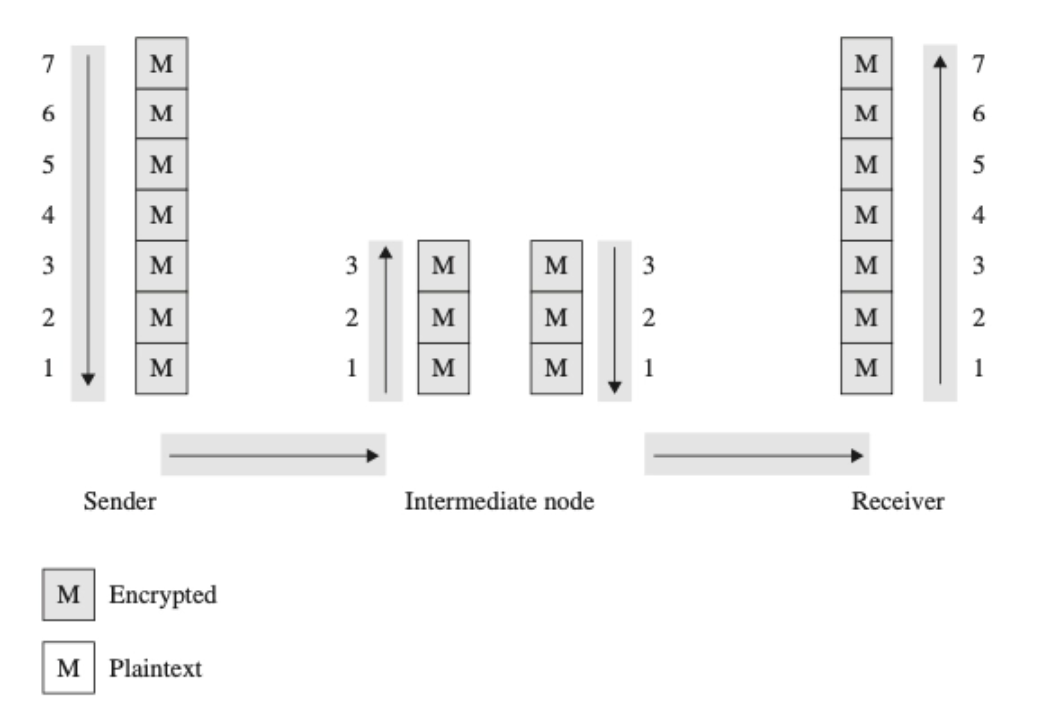
\includegraphics[width=0.7\textwidth]{Screenshot 2026-05-23 alle 11.03.47.png}
    \caption{Schema del modello OSI applicato all'End-to-End Encryption.}
    \label{fig:e2e_encryption}
\end{figure}

\subsection*{Crittografia del Browser}

I browser rappresentano un punto di accesso primario tra gli utenti e le risorse Internet, pertanto possono crittografare i dati per proteggerli durante la trasmissione. In questa sezione presentiamo due protocolli, SSH e SSL, entrambi in uso da decenni. Entrambi i protocolli consentono l'utilizzo di diversi algoritmi di crittografia e ammettono l'adozione di altri algoritmi nel tempo. Pertanto, anche se i vecchi schemi di crittografia (ad esempio, DES) dovessero cadere in disuso, qualsiasi applicazione basata su questi protocolli può essere aggiornata per utilizzare un algoritmo più recente e robusto.

\subsubsection*{Secure Shell (SSH)}

Nato nel 1995 per fornire un percorso sicuro, autenticato e crittografato per accedere all'interprete dei comandi (la "shell") di un sistema operativo da remoto. È lo strumento standard utilizzato dagli amministratori di sistema per gestire macchine a distanza o consegnare aggiornamenti di codice, andando a sostituire vecchie utilità non protette come Telnet, rlogin e rsh. Il suo compito è proteggere la comunicazione da attacchi di \textit{spoofing} (falsificazione) e da modifiche dei dati in transito. Quando due host si collegano tramite SSH, "negoziano" per scegliere quale algoritmo di crittografia usare (ad esempio DES o AES) e come autenticarsi a vicenda (tramite chiavi pubbliche o sistemi come Kerberos).

\subsubsection*{SSL e Cifratura TLS}

Progettato inizialmente a metà degli anni '90 per proteggere le comunicazioni tra browser e server web, il protocollo \textbf{Secure Sockets Layer (SSL)} ha attraversato diverse versioni fino alla 3.0 denominata \textbf{TLS (Transport Layer Security)}. SSL/TLS utilizza un sistema di "certificati" per l'autenticazione e per lo scambio delle chiavi crittografiche. A livello architetturale (modello OSI), si posiziona come un intermediario: sta sotto le applicazioni come i browser (livello 7) ma sopra le infrastrutture di base del TCP/IP (livelli inferiori). Crea un canale cifrato che garantisce l'autenticazione del server (sai con certezza a chi ti stai collegando) e viene usato non solo per la navigazione web, ma anche per proteggere email e trasferimenti di file.

\subsubsection*{Cypher Suite}

Quando un client (es. il tuo browser) e un server iniziano una connessione sicura tramite SSL/TLS, devono prima mettersi d'accordo su \textit{quali} strumenti matematici usare. Questo "pacchetto" di algoritmi scelti per gestire l'autenticazione, la cifratura della sessione e l'hashing prende il nome di \textbf{Cipher Suite}. Per permettere al protocollo di evolversi nel tempo (abbandonando gli algoritmi vecchi e adottando quelli nuovi), la scelta avviene tramite una \textbf{negoziazione}: il server invia una lista degli identificatori delle cipher suite che è in grado di utilizzare, e il client risponde selezionando la sua preferita da quell'elenco. (A volte avviene il contrario: il client propone una lista e il server sceglie l'algoritmo più forte che riesce a gestire).

% --- IMMAGINE TABELLA CYPHER SUITE ---
\begin{figure}[htbp]
    \centering
    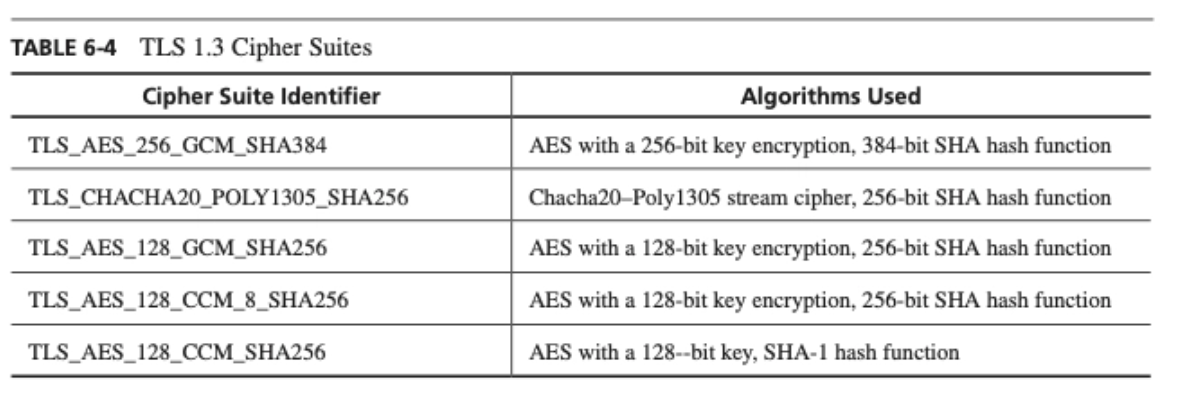
\includegraphics[width=0.9\textwidth]{Screenshot 2026-05-23 alle 11.03.59.png}
    \caption{Esempi di TLS 1.3 Cipher Suites.}
    \label{fig:cypher_suites}
\end{figure}

\subsection*{IPSec}

L'IPSec (Internet Protocol Security) non è un singolo protocollo, ma una complessa e potente suite di standard aperti sviluppata dall'IETF per garantire comunicazioni sicure su reti IP. A differenza di SSL/TLS che opera a livello applicativo o di trasporto, l'IPSec lavora al \textbf{Livello 3 (Rete)} del modello OSI. Questo significa che la sua protezione è completamente invisibile e trasparente per le applicazioni e per gli utenti: i pacchetti vengono cifrati e autenticati direttamente a livello di instradamento. Il cuore pulsante dell'architettura IPSec è il concetto di \textbf{Security Association (SA)}. Una SA è un accordo logico e matematico tra due dispositivi di rete (come due router o un computer e un firewall) che stabilisce esattamente come proteggere il traffico tra di loro. Per proteggere i dati, l'IPSec si affida a due protocolli distinti che possono essere usati singolarmente o combinati insieme, a seconda delle esigenze di sicurezza:

\begin{itemize}
    \item \textbf{AH (Authentication Header)}: Questo protocollo garantisce l'integrità dei dati, l'autenticazione dell'origine e la protezione contro gli attacchi di tipo "replay" (la ritrasmissione malevola di pacchetti catturati in precedenza). L'AH applica una firma crittografica matematica (MAC) non solo al carico utile del pacchetto (i dati veri e propri), ma anche a gran parte dell'intestazione IP originale. Tuttavia, l'AH \textbf{non fornisce alcuna cifratura}: i dati viaggiano sicuri da manipolazioni, ma rimangono leggibili in chiaro da chiunque intercetti il traffico.
    \item \textbf{ESP (Encapsulating Security Payload)}: A differenza dell'AH, l'ESP fornisce la \textbf{confidenzialità} crittografando il carico utile del pacchetto (solitamente tramite algoritmi simmetrici come l'AES). Oltre a cifrare, l'ESP garantisce anche l'autenticazione e l'integrità dei dati tramite un "trailer" aggiunto in fondo al pacchetto. Proprio per la sua capacità di rendere illeggibile il contenuto agli occhi di spie esterne, l'ESP è il protocollo alla base delle moderne reti private virtuali (VPN).
\end{itemize}

Ognuno dei protocolli visti sopra può essere configurato per operare in due modalità strutturalmente diverse, a seconda della tipologia di rete che si vuole creare.

Nella \textbf{Modalità Trasporto (Transport Mode)}, l'IPSec si limita a proteggere il carico utile del pacchetto originale, inserendo l'intestazione IPSec subito dopo l'intestazione IP originale e prima dei dati. In questo scenario, gli indirizzi IP originali del mittente e del destinatario rimangono visibili a tutti i router intermedi sulla rete. Questa modalità è molto leggera ed è pensata per le comunicazioni "End-to-End" dirette tra due host specifici (ad esempio, un amministratore che si collega in modo sicuro a un singolo server).

Nella \textbf{Modalità Tunnel (Tunnel Mode)}, invece, l'intero pacchetto IP originale (compresa la sua intestazione con gli indirizzi interni) viene completamente cifrato e incapsulato all'interno di un pacchetto IP totalmente nuovo. A questo nuovo pacchetto viene applicata una nuova intestazione IP esterna, che porta solitamente gli indirizzi pubblici dei due router o firewall di confine (i Security Gateway). Questa è la modalità standard utilizzata per creare le \textbf{VPN Site-to-Site}: un hacker che osserva il traffico su Internet vedrà solo un flusso di dati indecifrabile che viaggia tra due router aziendali, senza poter minimamente intuire quali e quanti computer stiano effettivamente comunicando all'interno delle due sedi.

% --- IMMAGINE STRUTTURA PACCHETTI IPSEC ---
\begin{figure}[htbp]
    \centering
    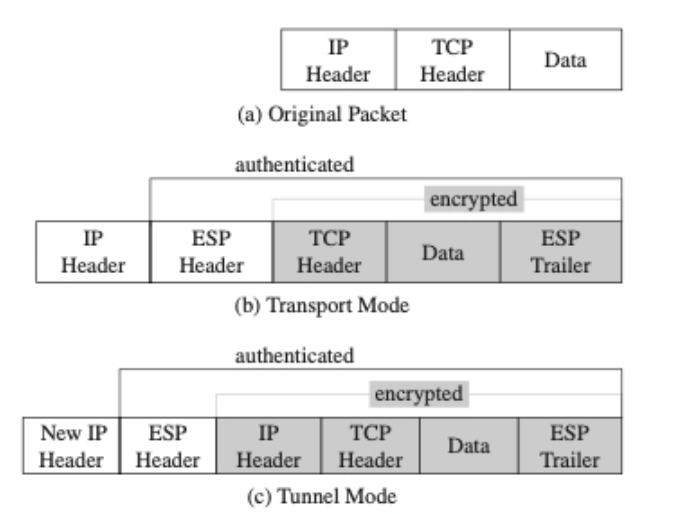
\includegraphics[width=0.7\textwidth]{Screenshot 2026-05-23 alle 11.04.06.png}
    \caption{Struttura dei pacchetti nelle modalità Transport e Tunnel.}
    \label{fig:ipsec_modes}
\end{figure}

Affinché i dispositivi possano stabilire queste complesse Security Association, hanno bisogno di scambiarsi le chiavi segrete e accordarsi sugli algoritmi in modo sicuro prima ancora di iniziare a trasmettere. Di questo si occupa l'\textbf{IKE (Internet Key Exchange)}. L'IKE è un protocollo di gestione e negoziazione che opera in due fasi: prima crea un canale di comunicazione di base sicuro (basato solitamente sullo scambio di chiavi Diffie-Hellman) e, successivamente, utilizza questo canale protetto per negoziare e generare in modo dinamico e automatico tutte le Security Association necessarie per far funzionare l'AH o l'ESP, cambiandole regolarmente nel tempo per massimizzare la sicurezza.

\subsection*{Firewalls}

Per comprendere la necessità di progettare i firewall, bisogna guardare all'evoluzione dei sistemi informativi. Storicamente, le reti aziendali nascevano come isole: piccole reti locali (LAN) completamente chiuse e isolate, intrinsecamente sicure perché irraggiungibili dall'esterno. Tuttavia, con l'avvento di Internet e delle reti geografiche (WAN), è emerso un forte paradosso organizzativo. Da un lato, c'è il forte desiderio, e la necessità di business, di connettere le proprie reti al mondo esterno per comunicare, scambiare dati e offrire servizi. Dall'altro lato, sorge la necessità altrettanto imperativa di limitare questo accesso per proteggere i dati sensibili, i sistemi e l'infrastruttura locale dalle innumerevoli minacce informatiche presenti sulla rete pubblica. Il firewall nasce esattamente come soluzione a questo conflitto: rappresenta un mezzo efficace per proteggere un sistema (o una rete di sistemi) dalle minacce esterne, garantendo al contempo la connettività vitale verso il mondo esterno.

% --- IMMAGINE FIREWALL EVOLUZIONE ---
\begin{figure}[htbp]
    \centering
    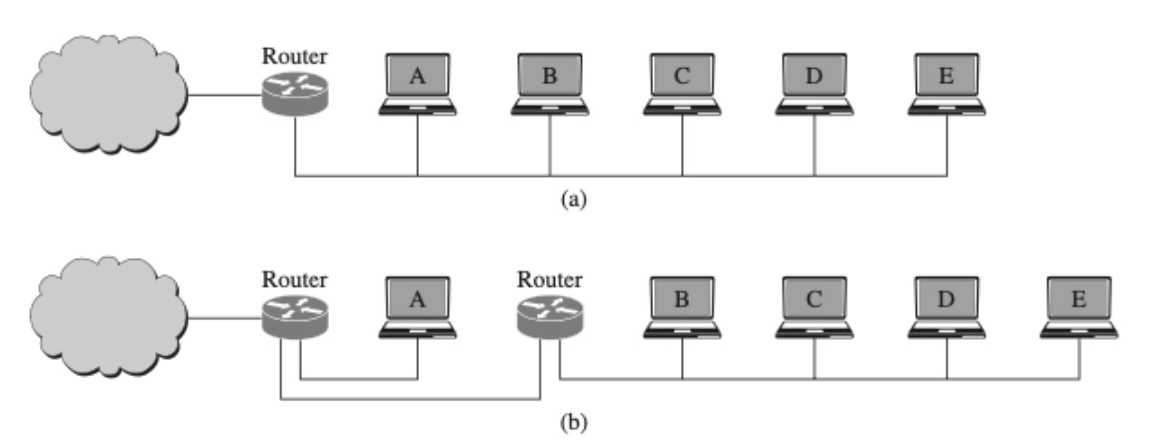
\includegraphics[width=0.8\textwidth]{Screenshot 2026-05-23 alle 11.04.14.png}
    \caption{Evoluzione delle reti e isolamento tramite firewall.}
    \label{fig:firewall_evoluzione}
\end{figure}

\subsubsection*{Principi Fondamentali e Policy di Accesso}

Un firewall funge da punto di strozzatura e di controllo (choke point) critico per la sicurezza informatica. Il suo ruolo principale è interconnettere reti che possiedono livelli di fiducia differenti, tipicamente separando una rete interna aziendale, considerata sicura, da una rete esterna non fidata come Internet. Per funzionare correttamente, la progettazione di un firewall deve rispettare due principi inviolabili: tutto il traffico in entrata e in uscita deve obbligatoriamente passare attraverso di esso, e solo il traffico esplicitamente autorizzato dalle policy di sicurezza locali può essere lasciato transitare. Poiché rappresenta la prima linea di difesa, il firewall stesso deve essere ospitato su un sistema operativo altamente blindato e immune alle intrusioni. Le decisioni di blocco o di passaggio si basano su specifiche caratteristiche o "policy di accesso", che possono valutare gli indirizzi IP, le porte di comunicazione, i protocolli applicativi, le identità degli utenti o i pattern di attività di rete.

% --- IMMAGINE FIREWALL CON POLICY ---
\begin{figure}[htbp]
    \centering
    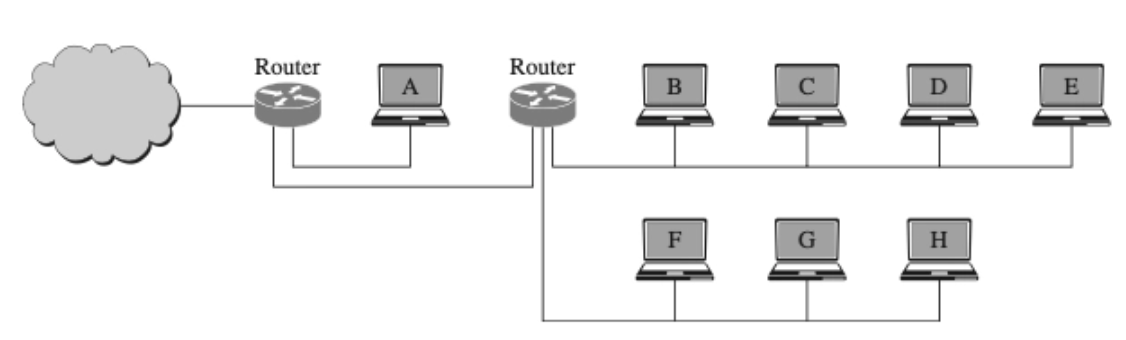
\includegraphics[width=0.8\textwidth]{Screenshot 2026-05-23 alle 11.04.20.png}
    \caption{Controllo del traffico basato su policy di accesso.}
    \label{fig:firewall_policy}
\end{figure}

Quando si configura un firewall, l'amministratore deve scegliere di adottare uno dei due approcci fondamentali, i quali definiscono l'atteggiamento di base della rete verso l'ignoto:

\begin{itemize}
    \item Default Deny (Quello che non è espressamente permesso è vietato): Blocca automaticamente tutto il traffico. Passa \textbf{solo} ciò che l'amministratore autorizza esplicitamente con una regola.
    \item Default Permit (Quello che non è espressamente vietato è permesso): Lascia passare automaticamente tutto il traffico. Blocca \textbf{solo} le minacce che l'amministratore vieta esplicitamente (una sorta di "lista nera").
\end{itemize}

Esistono diverse architetture (Packet Filtering, Stateful, Proxy) perché analizzano i dati a profondità diverse (Modello OSI). Un'analisi superficiale (come guardare solo gli indirizzi IP) è velocissima ma meno sicura; un'analisi profonda (leggere il contenuto dei pacchetti) è blindata ma rallenta pesantemente la rete. Si sceglie il tipo di firewall in base al giusto compromesso tra \textbf{sicurezza} e \textbf{prestazioni}.

\subsubsection*{Firewall a Filtraggio di Pacchetti (Packet-Filtering)}

La tipologia più basilare è il firewall a filtraggio di pacchetti, che opera esaminando individualmente ogni pacchetto IP in transito. Questo sistema prende la decisione di scartare (discard) o inoltrare (forward) il pacchetto confrontando esclusivamente le informazioni contenute nella sua intestazione (come l'indirizzo IP o la porta sorgente e destinazione) con un set di regole predefinite. A livello logico, un amministratore può configurare questo filtro secondo le due filosofie opposte viste pocanzi.

% --- IMMAGINE PACKET FILTERING ---
\begin{figure}[htbp]
    \centering
    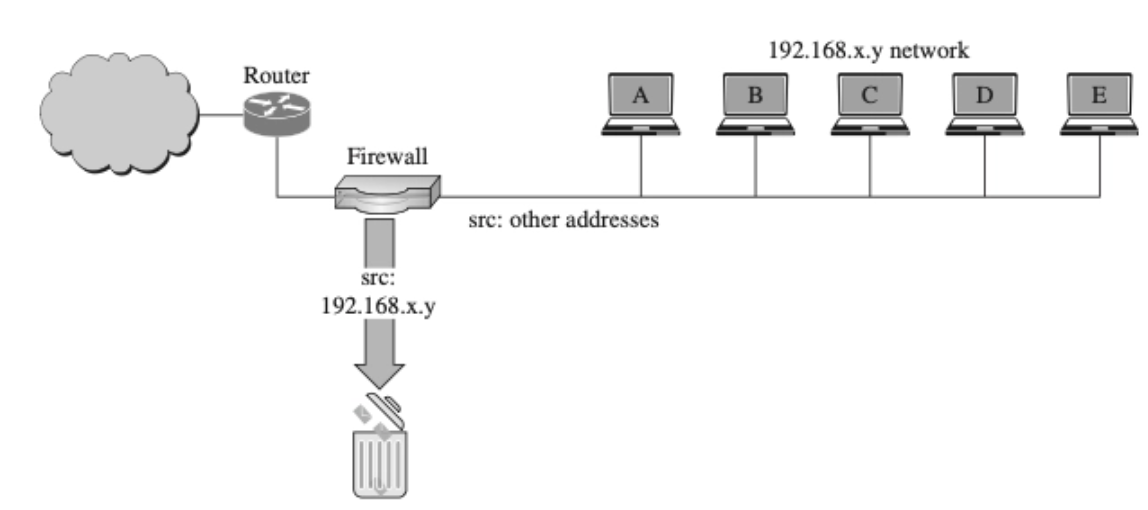
\includegraphics[width=0.8\textwidth]{Screenshot 2026-05-23 alle 11.04.27.png}
    \caption{Schema logico di un Firewall a Filtraggio di Pacchetti.}
    \label{fig:packet_filtering}
\end{figure}

\subsubsection*{I Gateway a Livello Applicativo e di Circuito (Proxy)}

Salendo di complessità troviamo i firewall basati su Proxy, che non si limitano a ispezionare il traffico, ma si interpongono attivamente nella comunicazione. L'\textbf{Application-Level Gateway} (o Application Proxy) funge da intermediario per specifici protocolli applicativi (come FTP o Telnet). Quando un utente interno vuole collegarsi all'esterno, si connette prima al gateway; quest'ultimo, dopo aver verificato le credenziali, apre una seconda connessione con il server remoto e fa da staffetta per i dati. Pur essendo estremamente sicuro, questo sistema analizza l'intero contenuto dei pacchetti, causando un notevole dispendio di risorse di calcolo (overhead). Il \textbf{Circuit-Level Gateway}, invece, opera in modo simile instaurando due connessioni TCP separate (una con l'utente e una con il server esterno), ma si limita a fare da passacarte per i segmenti di rete senza mai esaminarne il contenuto interno. Questa variante più leggera viene solitamente impiegata quando gli amministratori ripongono già un'elevata fiducia negli utenti della rete interna, preoccupandosi solo di nascondere la topologia della rete agli sguardi esterni.

% --- IMMAGINE CIRCUIT GATEWAY ---
\begin{figure}[htbp]
    \centering
    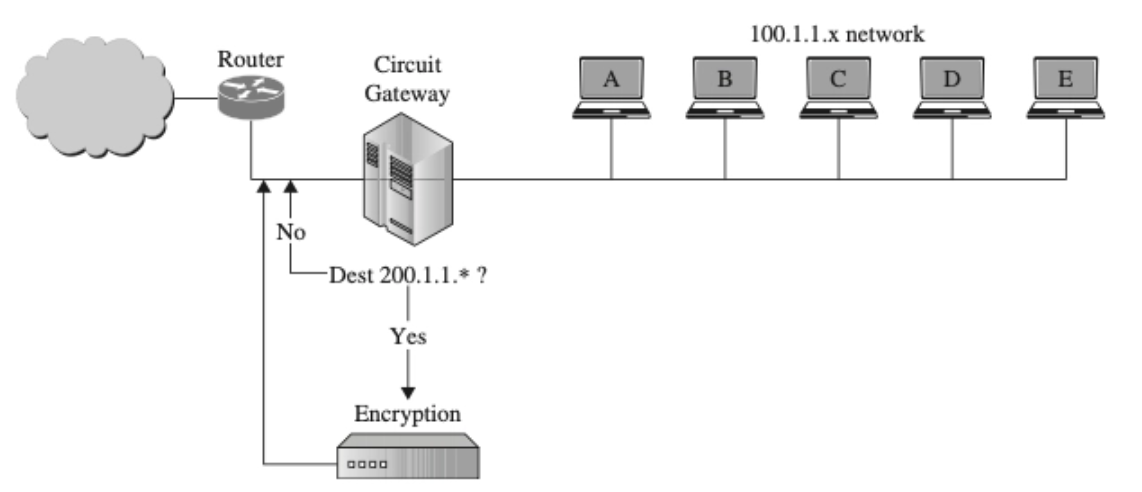
\includegraphics[width=0.8\textwidth]{Screenshot 2026-05-23 alle 11.04.35.png}
    \caption{Funzionamento di un Circuit Gateway Proxy.}
    \label{fig:circuit_gateway}
\end{figure}

\subsubsection*{Firewall a Ispezione di Stato (Stateful Inspection)}

Per ovviare ai limiti del filtraggio semplice, che analizza i pacchetti in modo isolato e "smemorato", è stato introdotto il firewall a ispezione di stato. Questo sistema rende le regole molto più stringenti, specialmente per il protocollo TCP, creando e mantenendo una vera e propria rubrica (directory) delle connessioni attive in uscita. Memorizzando lo "stato" di ogni conversazione appena stabilita dall'interno verso l'esterno, il firewall permette al traffico in entrata di attraversare le porte interne solo se i pacchetti in arrivo corrispondono al profilo esatto di una delle connessioni attualmente registrate in questa rubrica. In questo modo, i tentativi di connessione inattesi provenienti dall'esterno vengono bloccati sul nascere.

% --- IMMAGINE STATEFUL INSPECTION ---
\begin{figure}[htbp]
    \centering
    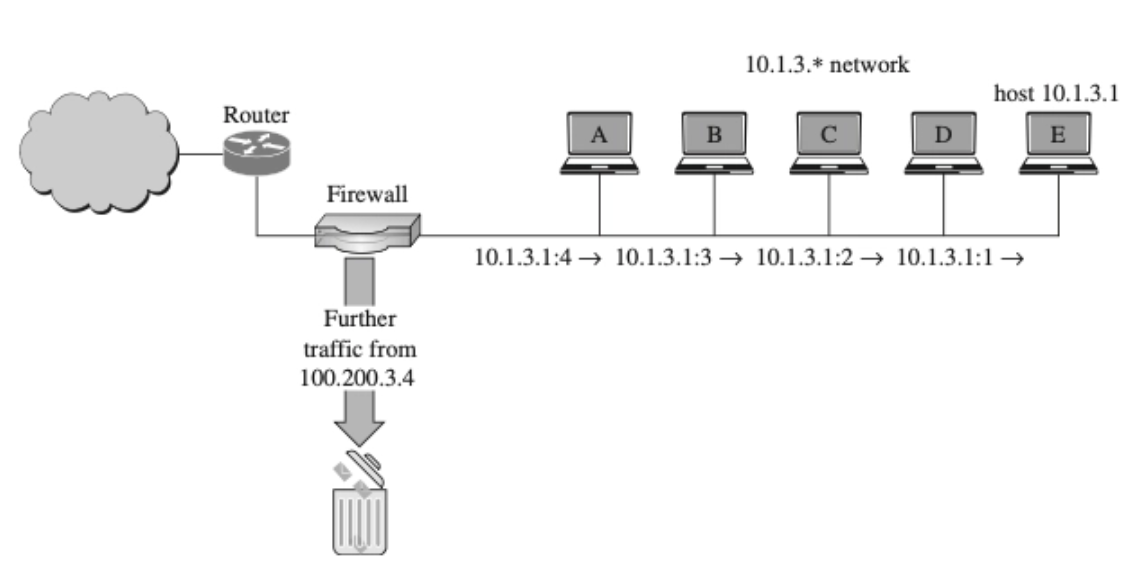
\includegraphics[width=0.8\textwidth]{Screenshot 2026-05-23 alle 11.04.41.png}
    \caption{Analisi delle sessioni in un Firewall Stateful.}
    \label{fig:stateful_inspection}
\end{figure}

\subsubsection*{Deep Packet Inspection (DPI)}

Mentre i firewall più semplici si limitano a leggere le "buste" dei pacchetti (indirizzi IP e porte), la Deep Packet Inspection apre la busta per analizzarne a fondo il contenuto, ovvero il carico utile (payload). Questa analisi profonda è fondamentale per bloccare gli hacker che cercano di infiltrare codice malevolo mimetizzandolo all'interno del traffico web legittimo, aggirando così i normali filtri. Incrociando dati provenienti da più livelli del pacchetto, la DPI permette di applicare policy estremamente granulari: un'azienda può usarla per bloccare l'invio verso l'esterno di documenti contenenti parole riservate (progetti segreti), oppure per analizzare il testo delle email in entrata e apporre in automatico l'etichetta "[External]" nell'oggetto, mettendo in guardia i dipendenti.

\subsubsection*{Application Proxy (Bastion Host)}

Salendo al massimo livello di controllo (il livello 7 del modello OSI), troviamo l'Application Proxy, spesso denominato "bastion host". Questo firewall funge da vero e proprio scudo intermedio "a due teste": blocca la connessione diretta tra l'utente esterno e il server interno, simulando di essere lui stesso l'applicazione finale. Quando riceve una richiesta, ad esempio via FTP per scaricare o caricare un file, il proxy controlla che il comando sia sintatticamente corretto e permesso dalle policy; se lo è, crea una nuova e separata connessione verso il server interno per eseguire l'operazione, inoltrando poi il risultato all'utente. Questa tecnica permette di manipolare ciò che l'esterno può vedere o fare: il proxy potrebbe permettere i comandi di download ma respingere silenziosamente quelli di upload, oppure ingannare l'utente nascondendo la reale struttura gerarchica delle cartelle del server interno.

% --- IMMAGINE BASTION HOST ---
\begin{figure}[htbp]
    \centering
    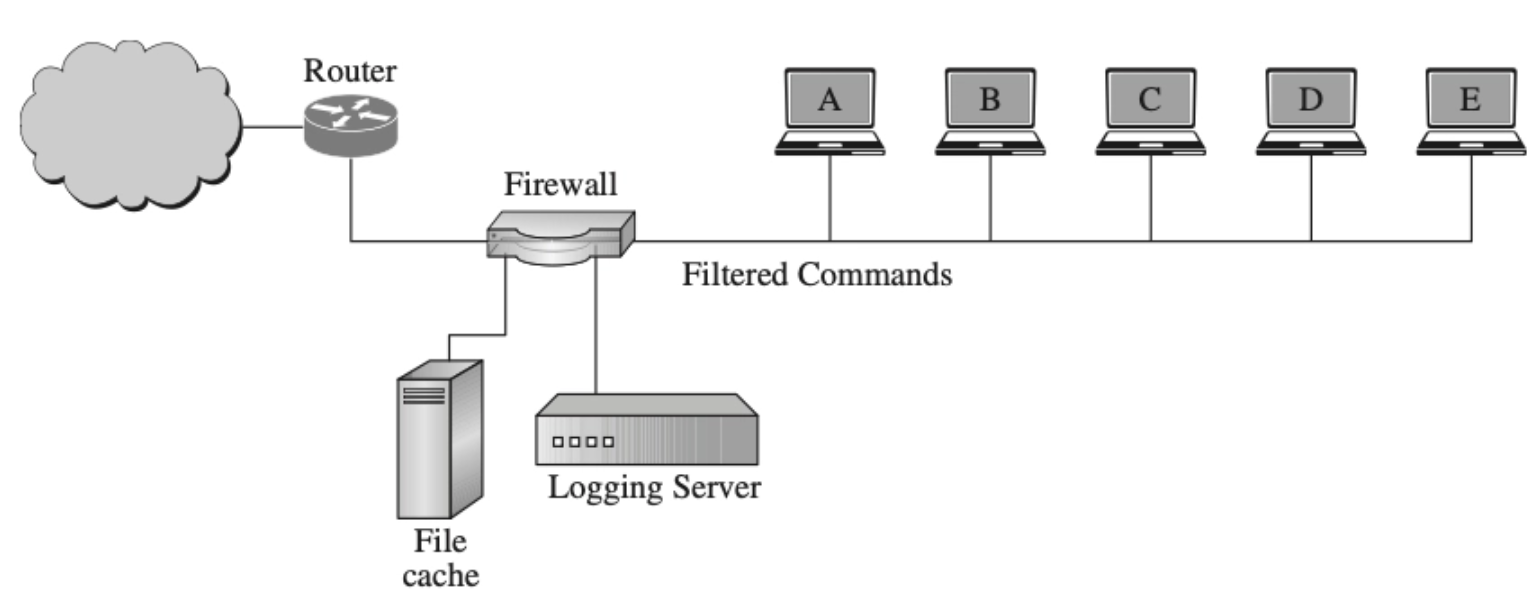
\includegraphics[width=0.8\textwidth]{Screenshot 2026-05-23 alle 11.04.46.png}
    \caption{Architettura di un Application Proxy (Bastion Host).}
    \label{fig:bastion_host}
\end{figure}

\subsubsection*{Il Guard}

Il "Guard" è la naturale e più potente evoluzione dell'Application Proxy. Mentre un proxy standard si limita a decidere se far passare o meno determinati comandi di un protocollo, il Guard può interpretare il flusso di dati, comprenderne il contesto (basandosi sull'identità dell'utente o su interazioni precedenti) e modificarlo per ottenere risultati complessi, eseguendo di fatto un codice di programmazione vero e proprio. Le applicazioni pratiche di un Guard sono vastissime: può limitare a una scuola la banda per contenuti multimediali preservando quella per i testi, può bloccare un utente universitario che tenta di inviare troppe email in un lasso di tempo troppo breve, può fungere da "paywall" per un giornale online recapitando solo l'anteprima testuale di un articolo, oppure può intercettare tutti i file in ingresso e dirottarli automaticamente verso uno scanner antivirus prima di consegnarli all'utente.

\subsubsection*{Sandbox}

L'ultimo meccanismo difensivo esaminato è la Sandbox. Quando un firewall intercetta del codice eseguibile in entrata o un allegato sospetto, invece di lasciarlo eseguire direttamente sul computer dell'utente interno con il rischio di causare danni, lo esegue all'interno di un ambiente virtuale e totalmente isolato dal resto della rete. Solo se, dopo essere stato osservato nella sandbox, il codice dimostra di avere un comportamento innocuo, gli viene permesso l'accesso alla zona protetta. Questa scala evolutiva (dai filtri di pacchetti, ai proxy, fino ai guard e alle sandbox) dimostra un principio cardine: man mano che ci si sposta da decisioni meccaniche a ispezioni analitiche vicine all'intelligenza artificiale, si aumenta drasticamente la sicurezza ma si richiede esponenzialmente più tempo di elaborazione, impattando sulle performance globali della rete.

% --- IMMAGINE SANDBOX ---
\begin{figure}[htbp]
    \centering
    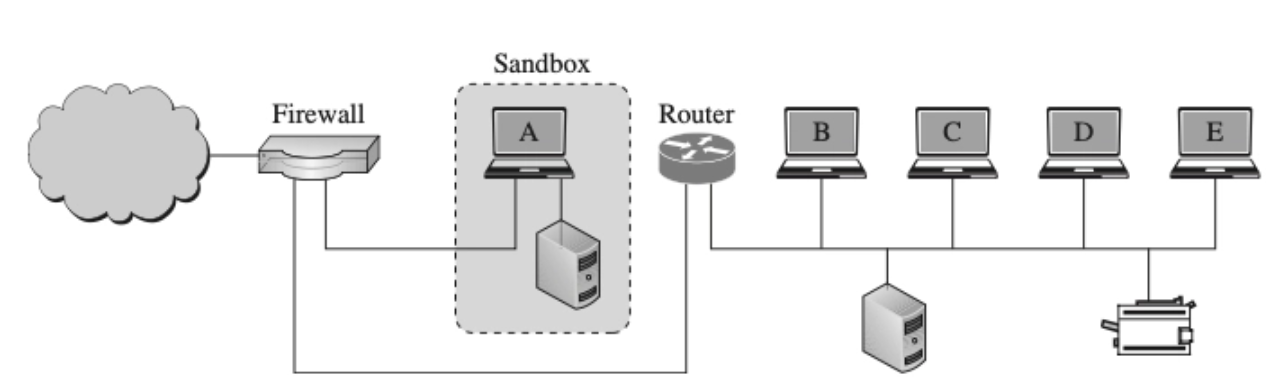
\includegraphics[width=0.8\textwidth]{Screenshot 2026-05-23 alle 11.04.53.png}
    \caption{Isolamento dell'esecuzione tramite Sandbox.}
    \label{fig:sandbox}
\end{figure}

\subsubsection*{I Limiti Intrinseci dei Firewall}

Un firewall è efficace \textit{esclusivamente} se controlla l'intero perimetro della rete. Se all'interno dell'azienda esiste anche solo una connessione non mediata (ad esempio, un dipendente che collega un access point wireless non autorizzato o un modem personale alla rete interna) l'intero sistema diventa vulnerabile, poiché l'attaccante può bypassare completamente il firewall. Inoltre, i firewall sono il punto di contatto più visibile dall'esterno, rendendoli di fatto il bersaglio primario per gli hacker. Sebbene siano progettati per resistere agli attacchi (spesso vengono spogliati di strumenti software come compilatori o linker per evitare che un intruso li usi se prende il controllo), non sono impenetrabili e richiedono una configurazione costantemente aggiornata e una revisione periodica dei log di sistema. Infine, un firewall ha un controllo solo parziale sul contenuto profondo dei dati ammessi. Una volta che un dato legittimo supera il perimetro, il firewall non può più proteggerlo. Per questo motivo, il codice malevolo o i dati corrotti devono essere gestiti da altri sistemi interni, seguendo il principio fondamentale della \textbf{difesa in profondità} (defense in depth): non affidarsi mai a un solo livello di sicurezza, ma stratificare più difese.

\subsection*{Il Ruolo del NAT (Network Address Translation)}

Il \textbf{NAT} è una tecnologia vitale per la sicurezza e la gestione degli indirizzi di rete. Il problema che il NAT risolve è l'esposizione degli indirizzi IP interni: se i computer di un'azienda comunicassero su Internet usando i propri indirizzi IP reali, un attaccante esterno potrebbe facilmente mappare la topologia della rete, scoprendo quanti dispositivi ci sono e come sono collegati. Una volta noti, questi indirizzi sarebbero sfruttabili per sempre.

Il dispositivo NAT (spesso integrato nel router o nel firewall di confine) funge da intermediario. Quando un computer interno (es. con IP privato 192.168.1.5) invia una richiesta verso Internet, il NAT intercetta il pacchetto e ne altera l'intestazione, sostituendo l'indirizzo IP privato con il proprio indirizzo IP pubblico (es. 171.203.129.98). Il mondo esterno "vede" esclusivamente l'IP pubblico del NAT, mantenendo la vera identità e la struttura della rete locale completamente nascoste e protette dagli sguardi indiscreti.

% --- IMMAGINE NAT ---
\begin{figure}[htbp]
    \centering
    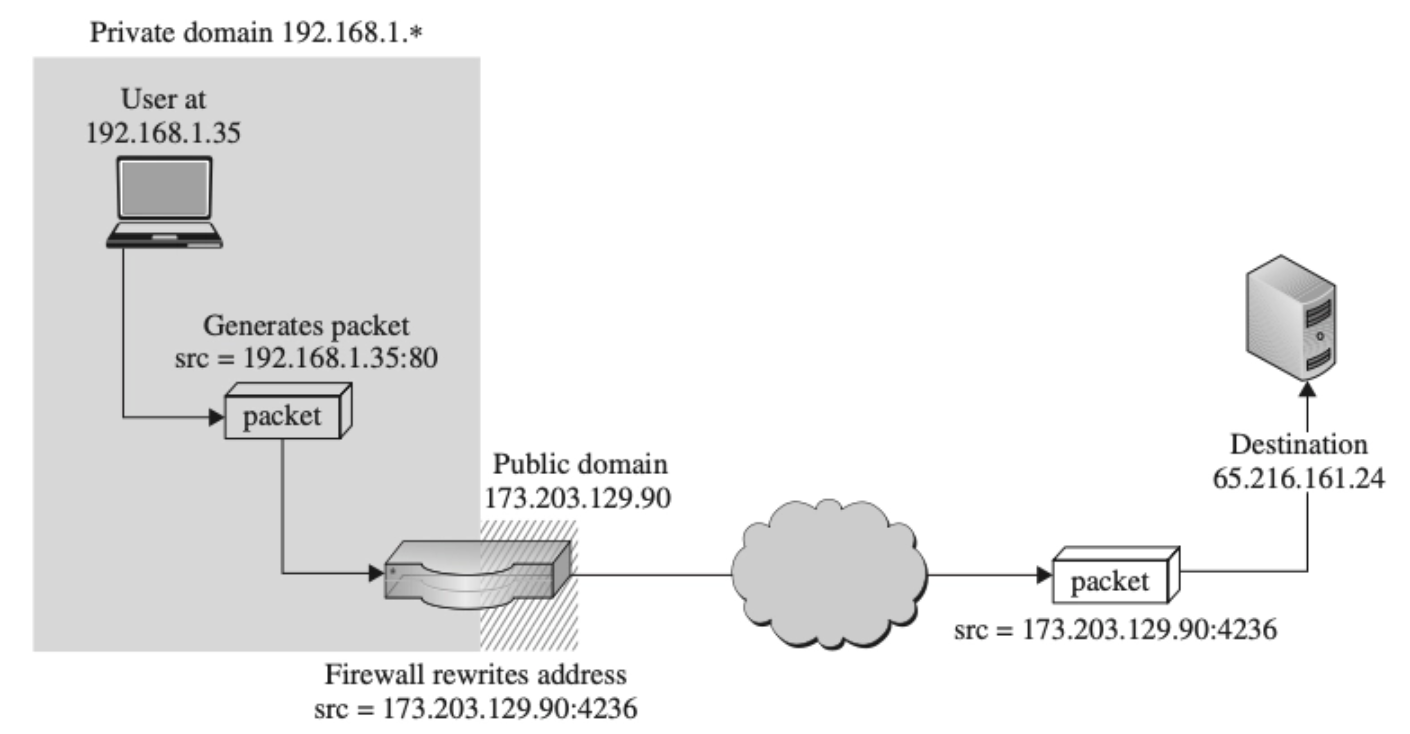
\includegraphics[width=0.8\textwidth]{Screenshot 2026-05-23 alle 11.04.59.png}
    \caption{Traduzione degli indirizzi di rete tramite NAT.}
    \label{fig:nat_diagram}
\end{figure}

\subsection*{Intrusion Detection e Prevention}

Mentre i controlli perimetrali come i firewall agiscono in modo preventivo bloccando le azioni dannose note all'ingresso, non possono nulla contro gli utenti interni che abusano dei propri privilegi o contro estranei che sono già riusciti a eludere i controlli di accesso. In questo contesto si inserisce l'\textbf{Intrusion Detection System (IDS)}, che rappresenta la successiva e fondamentale linea di difesa. L'IDS è un dispositivo (o un software) progettato per monitorare costantemente l'attività del sistema e della rete allo scopo di identificare eventi sospetti o palesemente malevoli. Il suo funzionamento si basa sulla ricezione di dati grezzi dai sensori, sulla loro analisi e sull'attivazione di un allarme al verificarsi di specifiche condizioni, demandando poi la risposta attiva a un team umano o a piani di emergenza predefiniti. Se il sistema viene configurato per passare in "modalità protezione" e intervenire direttamente sul traffico (ad esempio riconfigurando elettronicamente un segmento di rete per isolare l'intruso) assume invece la denominazione di \textbf{Intrusion Prevention System (IPS)}. Le funzioni di base di un IDS spaziano dal monitoraggio delle attività degli utenti, alla revisione delle configurazioni di sistema alla ricerca di vulnerabilità, fino al riconoscimento di pattern di attacco noti.

\subsubsection*{Le due Metodologie di Rilevamento}

Per svolgere il proprio compito analitico, i sistemi IDS si dividono in due grandi tipologie basate sull'approccio utilizzato:


\textbf{1. Rilevamento Signature-Based (Basato su Firme):} Questo approccio funziona attraverso un meccanismo di \textit{pattern-matching}: l'IDS confronta il traffico di rete o le attività di sistema con un database preesistente di "firme", ovvero modelli che descrivono le caratteristiche precise di attacchi già noti. Ad esempio, l'IDS può riconoscere facilmente un port scan individuando una specifica sequenza temporale di pacchetti TCP SYN inviati in rapida successione a porte diverse dalla medesima sorgente.

Sebbene sia efficiente, questo sistema presenta due gravi vulnerabilità teoriche e pratiche. In primo luogo, è del tutto inefficace contro attacchi nuovi (zero-day) per i quali non è ancora stata creata e installata una firma. In secondo luogo, un attaccante consapevole può facilmente ingannare l'IDS alterando leggermente la forma del proprio attacco: modificando le lettere in maiuscolo, codificando gli spazi come "\%20" o alterando l'ordine dei pacchetti, l'attaccante fa fallire la corrispondenza esatta con la firma nel database. Questo costringe l'IDS a dover "normalizzare" il traffico per riconoscerlo, riducendone le prestazioni.

Un'ulteriore evoluzione di questo approccio è la \textbf{Stateful Protocol Analysis}. Il rilevamento a firme tradizionale fatica quando il pattern di attacco non è racchiuso in un singolo pacchetto, ma è lungo e variabile nel tempo (come un attacco DoS di tipo SYN Flood, basato su connessioni lasciate a metà). Per riconoscere queste firme complesse, l'IDS opera come una vera e propria macchina a stati (State Machine): non si limita a leggere i pacchetti isolati, ma memorizza l'intera "storia" della conversazione TCP, tenendo traccia dei passaggi (es. SYN ricevuto, SYN-ACK inviato, in attesa di ACK). Se una connessione va in timeout una sola volta viene considerata un errore di rete, ma se questa transizione incompleta si ripete sistematicamente, il sistema riconosce il pattern d'attacco. L'efficacia di questa tecnica ha però un altissimo costo computazionale: dovendo tracciare simultaneamente lo stato esatto di decine di migliaia di connessioni parallele, il sistema richiede una quantità enorme di memoria e risorse di calcolo.

\textbf{2. Rilevamento Heuristic (Euristico o Anomaly-Based):} Per superare i rigidi limiti del rilevamento tramite firme (incapaci di scovare attacchi nuovi), i sistemi euristici abbandonano la ricerca di schemi di attacco specifici per concentrarsi sulla ricerca di comportamenti fuori dall'ordinario. L'IDS costruisce preliminarmente un modello del comportamento "normale" e accettabile di un utente o di un sistema; da quel momento in poi, qualsiasi azione che si discosti in modo significativo da tale linea di base viene contrassegnata come sospetta.

Il cuore di questo sistema è un motore di inferenza che impara a correlare gli eventi nel tempo, e lo fa operando principalmente in due modi distinti:

\begin{itemize}
    \item \textbf{L'approccio State-based (Basato sullo stato):} I sistemi di rilevamento delle intrusioni \textit{state-based} osservano il sistema mentre attraversa continui cambiamenti del suo stato generale o della sua configurazione, passando progressivamente da una condizione "pulita" (clean) a una compromessa o "sporca" (dirty). Piuttosto che allarmarsi per un singolo evento isolato, l'IDS cerca di rilevare quando l'intero sistema devia inesorabilmente verso modalità insicure.
    \item \textbf{L'approccio Model-based (Basato sui modelli):} In alternativa, il motore di inferenza può operare costruendo un modello dinamico del comportamento, capace di adattarsi alle variazioni e all'evoluzione delle azioni di una persona nel corso del tempo. Questa tecnica confronta l'attività reale in corso con una rappresentazione nota di "normalità" creata su misura.
\end{itemize}

Un esempio di questo rilevamento che sfrutta l'approccio State-Based è il seguente:

Inizialmente, il Computer A inizia a ispezionare gli altri computer della rete locale per cercare aree di archiviazione o file disponibili agli utenti. Nella prima fase, A sonda il Computer B. Il Computer B rifiuta l'accesso. L'IDS classifica questo singolo evento come "insolito", ma non lancia alcun allarme: si limita a prendere nota del tentativo di accesso negato, poiché potrebbe trattarsi di un semplice errore o di un'operazione benigna. Poco dopo, il Computer A sonda un altro nodo, il Computer C. Questo secondo tentativo rende il comportamento "più insolito" agli occhi dell'IDS. Il Computer C, a differenza del precedente, ha una struttura di directory aperta e il Computer A riesce a ottenere l'elenco di tutti i file accessibili. A questo punto, il livello di guardia si alza e l'IDS contrassegna formalmente l'attività come \textbf{sospetta}. La fase finale avviene quando il Computer A tenta di copiare in blocco tutti i file appena trovati sul Computer C. A questo punto, l'IDS riconosce che l'intera sequenza logica rappresenta un probabile attacco (come un tentativo di esfiltrazione o furto di dati) e fa finalmente scattare l'allarme allertando l'amministratore di sistema.

\subsubsection*{Posizionamento Logico: Front-End vs. Internal IDS}

Un aspetto fondamentale nella progettazione di un'architettura di sicurezza è il posizionamento dell'IDS, che determina quali minacce il sistema sarà in grado di "vedere".

Un \textbf{Front-end IDS} viene collocato esattamente all'ingresso della sottorete, intercettando e analizzando tutti i pacchetti provenienti dall'esterno prima che vi facciano il loro ingresso. Funzionando da sentinella perimetrale (e per questo spesso integrato direttamente nel firewall), ha il vantaggio di poter bloccare il traffico dannoso sul nascere, causando solo un lievissimo e impercettibile rallentamento nel flusso dei dati. Tuttavia, la sua esposizione verso l'esterno lo rende un bersaglio primario: gli hacker sanno che abbattere questa singola difesa rende l'intera rete più vulnerabile. Il limite critico del Front-end IDS è però la sua totale cecità verso l'interno: non può rilevare minacce originate direttamente da macchine interne già infette, né accorgersi se un computer compromesso sta attaccando lateralmente un altro host della stessa rete.

Per colmare questa pericolosa lacuna si utilizza un \textbf{Internal IDS}, progettato esclusivamente per monitorare il traffico locale tra le macchine aziendali. Se un hacker esterno invia pacchetti apparentemente innocui per ordinare a un computer interno compromesso di lanciare un attacco DoS contro il server aziendale, la sentinella frontale non se ne accorgerà, ma l'Internal IDS sì. Oltre a essere invisibile e quindi ben protetto dagli attacchi diretti da Internet, questo sistema interno è nella posizione ideale per apprendere le normali abitudini quotidiane degli utenti (tramite approccio euristico) e segnalare tempestivamente qualsiasi anomalia comportamentale.

\subsubsection*{Ambito di Protezione: Host-Based vs. Network-Based (HIDS vs NIDS)}

Oltre a dove vengono posizionati, i sistemi di rilevamento si distinguono radicalmente per il loro ambito d'azione e per la loro natura fisica o software.

L'\textbf{Host-Based IDS (HIDS)} è un programma software installato e in esecuzione su un singolo computer o server. Il suo unico scopo è proteggere la macchina su cui risiede, raccogliendo e analizzando dati strettamente locali forniti dal sistema operativo, come i file di registro (log), le richieste di accesso alle risorse sensibili e le applicazioni eseguite. Il difetto principale dell'HIDS è la sua vulnerabilità intrinseca: essendo un normale processo in esecuzione sul computer bersaglio, se un intruso riesce a ottenere privilegi elevati su quella macchina può facilmente individuare l'HIDS e spegnerlo, disattivando di colpo tutte le difese.

Al contrario, il \textbf{Network-Based IDS (NIDS)} è solitamente un dispositivo hardware dedicato (appliance) che "ascolta" il traffico di intere sezioni della rete per proteggere contemporaneamente tutti i computer a essa collegati. Il NIDS analizza i volumi di traffico e il contenuto dei pacchetti in transito cercando attività insolite e attacchi trasversali. Il grandissimo vantaggio del NIDS rispetto alla controparte host risiede nella sua formidabile capacità di autodifesa: potendo operare in modalità puramente passiva --- limitandosi a osservare i dati sul cavo di rete senza mai trasmettere pacchetti propri --- risulta del tutto invisibile. In questo modo, un attaccante non ha alcun modo di sapere di essere sotto osservazione e non può mirare al NIDS per neutralizzarlo.

\subsubsection*{Obiettivi di Progettazione e Sfide Operative: Stealth Mode e Accuratezza}

Un IDS ideale dovrebbe essere, per definizione, veloce, semplice, accurato, rigoroso e completo: deve cioè garantire la massima capacità di rilevamento senza impattare negativamente sulle prestazioni della rete (overhead). Per avvicinarsi a questo standard, il design di un IDS moderno integra diverse strategie, come il filtraggio in tempo reale a livello di intestazione e di contenuto, il mantenimento dello stato delle connessioni e l'utilizzo di finestre temporali scorrevoli per correlare eventi apparentemente slegati. Tuttavia, per essere realmente efficace, questo strumento deve affrontare due sfide operative cruciali: la protezione della propria integrità e la calibrazione della propria precisione. Poiché un IDS rappresenta il primo bersaglio logico per un attaccante che desidera operare indisturbato, esso deve operare in \textbf{Stealth Mode} (Modalità Furtiva): la sua interfaccia di monitoraggio deve essere configurata per ascoltare passivamente il traffico senza mai inviare pacchetti in rete e senza possedere un indirizzo IP pubblicato, rendendo il dispositivo di fatto invisibile e protetto da attacchi diretti. Parallelamente, il sistema deve gestire il delicato problema dell'\textbf{accuratezza}, trovando un equilibrio precario tra due errori opposti: il \textit{Falso Positivo}, che genera allarmi per attività innocue frustrando gli amministratori e portandoli a ignorare il sistema, e il \textit{Falso Negativo}, che permette a una minaccia reale di passare inosservata. Poiché non esiste una configurazione perfetta, il compito dell'amministratore è calibrare continuamente la sensibilità del sistema, consapevole che, in ultima istanza, l'IDS non è uno strumento autonomo ma un supporto che richiede l'intervento umano per monitorare i risultati e rispondere concretamente agli allarmi generati.

\subsubsection*{I Limiti dell'IDS}

Per concludere la panoramica, bisogna interiorizzare i limiti intrinseci di questi strumenti. Un IDS non pensa: si limita a cercare debolezze conosciute, che siano schemi rigidi (firme) o deviazioni statistiche da modelli pre-calcolati (euristica). Ma la limitazione assoluta e più importante riguarda la sua operatività: un IDS non è in grado di agire da solo. Raccogliere dati, identificare anomalie e far scattare sirene digitali è completamente inutile se non c'è una controparte umana pronta a monitorare quello storico e a rispondere fisicamente agli allarmi. Un'installazione non presidiata è, a tutti gli effetti, un investimento a vuoto.

\subsubsection*{Dall'IDS all'IPS: La risposta attiva}

Il limite principale di un IDS è che, pur essendo eccellente nell'identificare un attacco, rimane un sistema passivo: genera un avviso, ma non ferma l'aggressore. L'\textbf{IPS (Intrusion Prevention System)} colma questa lacuna integrando funzioni di risposta automatica. L'obiettivo non è più solo rilevare, ma bloccare o mitigare il danno in tempo reale.

Quando un IPS rileva un'attività malevola, può attivare diverse strategie di risposta, che si muovono su un gradiente di intensità crescente:

\begin{itemize}
    \item \textbf{Monitoring (Monitoraggio):} È la risposta più prudente. Il sistema continua a osservare, magari aumentando la granularità dei dati raccolti per analizzare meglio l'attacco, ma non intraprende azioni visibili per non allertare l'attaccante che ha scoperto la sua presenza. È ideale nella fase iniziale di studio della minaccia.
    \item \textbf{Protecting (Protezione):} Qui l'IPS interviene attivamente per ridurre l'esposizione al rischio. Questo include l'aumento dei controlli di accesso, la rimozione temporanea di una risorsa dalla rete o la chiusura forzata della connessione utilizzata dall'attaccante. Spesso queste azioni sono intenzionalmente visibili all'aggressore: l'obiettivo è scoraggiarlo, mostrandogli che la sua attività è stata rilevata e bloccata, spingendolo a desistere e cercare un bersaglio più facile.
    \item \textbf{Signaling (Segnalazione):} L'IPS invia un segnale di allerta ad altri componenti del sistema di difesa (come un firewall o un router), permettendo a tutta l'infrastruttura di coordinarsi per contrastare la minaccia in modo corale.
    \item \textbf{Call a human (Allerta umana):} È la risposta estrema, in cui il sistema richiede l'intervento diretto di un amministratore umano per valutare decisioni complesse che il software non può gestire autonomamente.
\end{itemize}

Una caratteristica peculiare dell'IPS è come possa adottare comportamenti \textbf{adattivi}, reagendo in modo dinamico all'evoluzione dell'attacco. Se un attacco è di tipo \textit{Denial of Service} (inondazione di traffico), l'IPS non si limita a bloccare, ma può attuare strategie complesse: può reindirizzare il traffico verso un host di monitoraggio (una sorta di "trappola" o \textit{honeypot}), può tentare di aumentare la capacità della rete aggiungendo host online per bilanciare il carico, oppure può limitare le performance rallentando deliberatamente alcuni tipi di traffico per dare priorità a quelli vitali. Nei casi in cui la minaccia è troppo grave e rischia di compromettere l'intera infrastruttura, l'IPS può adottare le misure più drastiche: negare l'accesso a specifici servizi, spegnere segmenti della rete locale o, nei casi peggiori, decidere di isolare completamente l'intera rete aziendale dal mondo esterno, sacrificando la connettività per proteggere l'integrità dei dati aziendali.

\end{document}

